\documentclass[titlepage=true]{scrartcl}

% !TEXroot=main.tex
\usepackage{enumitem}
\usepackage[german]{babel}
%\usepackage{polyglossia}
%\setmainlanguage[babelshorthands=true]{german}
%\setotherlanguage{english}

%\setkomafont{chapter}{\normalfont\Large\itshape} only koma classes (src...)

%Wichtig: danach
\usepackage{blindtext}
\usepackage{float}
\usepackage{listings}

\usepackage{amsmath}
\usepackage{mathtools}

\usepackage{graphicx}
%\usepackage{tabu}
\usepackage{booktabs}
\usepackage{multicol}
\usepackage{amsfonts} 

\usepackage{amssymb}    % Mathematische Symbole
\usepackage{booktabs}   % Korrekter Tabellensatz
\usepackage[hang,font={sf,footnotesize},labelfont={footnotesize,bf}]{caption}

\usepackage[% Seitenlayout anzeigen
left=2.5cm,
right=2.5cm,
top=2.5cm,
bottom=2cm,
%includeheadfoot
]{geometry}

%\usepackage{hyperref}
\usepackage{subcaption}
\usepackage{lscape}
\usepackage{rotating}
\usepackage{pdflscape}
\usepackage{graphicx}


\usepackage[
detect-all,
locale=DE,
binary-units=true,
range-phrase={\,\dots\,},
]{siunitx}                % Größen mit Einheiten korrekt darstellen
\DeclareSIUnit{\Bit}{Bit}

% Hyperref sollte sehr spät eingebunden werden, da es viele
% Elemente modifiziert
\usepackage{hyperref}  % Hyperlinks
\usepackage{color}
% Farben definieren
\definecolor{linkblue}{RGB}{0, 0, 100}
\definecolor{linkblack}{RGB}{0, 0, 0}
\definecolor{comment}{RGB}{63, 127, 95}
\definecolor{darkgreen}{RGB}{14, 144, 102}
\definecolor{darkblue}{RGB}{0,0,168}
\definecolor{darkred}{RGB}{128,0,0}
\definecolor{javadoccomment}{RGB}{0,0,240}

% Einstellungen für das Hyperref-Paket
\hypersetup{
	colorlinks=true,      % Farbige links verwenden
	%    allcolors=linkblue,
	%    allcolors=black,
	linktoc=all,          % Links im Inhaltsverzeichnis
	linkcolor=linkblack,  % Querverweise
	citecolor=linkblack,  % Literaturangaben
	filecolor=linkblack,  % Dateilinks
	urlcolor=linkblack,   % URLs
	pdfstartpage=1
}


\usepackage{eso-pic}
% Makros für typographisch korrekte Abkürzungen
\newcommand{\zb}[0]{z.\,B.\ }
\newcommand{\dahe}[0]{d.\,h.\ }
\newcommand{\ua}[0]{u.\,a.\ }
\newcommand{\tus}[0]{\textunderscore}
% Diese Zusammensetzungen bestehen jeweils aus zwei Wörtern.
% Daher muss ein Leerzeichen dazwischen stehen. Traditionell
% wird das durch einen kleinen Abstand realisiert.

\title{Kartierung eines und Navigation in einem Labyrinth}
\author{\textit{David Siekacz}}
\date{16. August 2022}

%\subtitle{Die AG-Dokumentation der Feld- Wald und Wiesenbiologie AG beinhaltet Forschungsergebnisse aus dem ganzen Labjahr}
%\titlehead{Hochschule Mannheim, Hector-Seminar}
\subject{Kooperationsprojekt}
\publishers{Betreut durch Prof. Dr. Thomas Ihme}
\AddToShipoutPicture*
{%
	\put(100,700)%the specific point of the page with coordinates (x=100, y=100)
	{
\includegraphics[scale=0.3]{Bilder/HSMA-Logo.png}}%
}
\AddToShipoutPicture*
{%
	\put(400,700)%the specific point of the page with coordinates (x=100, y=100)
	{
\includegraphics[scale=0.4]{Bilder/hector-seminar_logo.jpg}}%
}
%numeric, authortitle
%\usepackage[style=authoryear, backend=biber]{biblatex}
\usepackage[defernumbers=true,backend=biber,
isbn=false,                  % ISBN nicht anzeigen, gleiches geht mit nahezu
% allen anderen Feldern
autocite=inline,             % regelt Aussehen für \autocite
%      inline: Zitat in Klammern (\parancite)
%      footnote: Zitat in Fußnoten (\footcite)
%      plain: Zitat direkt ohne Klammern (\cite)
style=ieee,       % Legt den Stil für die Zitate fest
%      ieee: Zitate als Zahlen [1]
%      alphabetic: Zitate als Kürzel und Jahr [Ein05]
%      authoryear: Zitate Author und Jahr [Einstein (1905)]
hyperref=true,                  % Hyperlinks für Zitate
citestyle=numeric-comp,         % Fasst Nummernzitate zusammen [1-7, 10]
natbib=true                     % Komatibilität zu natbib
]{biblatex}  
\addbibresource{literaturreferenzen.bib}

\begin{document}
	\maketitle
	\KOMAoptions{titlepage=false}
	% !TEXroot=main.tex
\renewcommand\abstractname{Zusammenfassung} 
\begin{abstract}
	{\large\textbf{\abstractname:}} \newline
	Die Robotik nimmt ein immer größer werdendes Forschungsgebiet innerhalb der Wissenschaft ein. Roboter werden für unser alltägliches Leben immer wichtiger. Doch um sich in unser Umfeld, \zb als Staubsaugroboter, integrieren zu können, müssen diese auch in der Lage sein, in Umgebungen zu navigieren.
	Dieser Projekt handelt von der Kartierung und darauf aufbauenden Navigation innerhalb eines unbekannten Labyrinthes. Wie  Menschen zum Finden eines Ortes eine Karte brauchen, so benötigen auch Roboter diese, um zu navigieren. Dazu wird das Robot-Operating-System genutzt, um den Roboter, einen Turtelbot, diese Aufgaben bewältigen zu lassen. Dazu kartiert dieser ein Labyrinth, kreiert eine Karte, durch welcher der Roboter schlussendlich eigenständig in jenem Labyrinth navigieren kann. 
\end{abstract}
	\newpage
	\tableofcontents
	\newpage
	%% !TEXroot=main.tex
\section{ROS}
{
	\subsection{Überblick}
	{
		Das sogenannte Robot Operating System, kurz ROS genannt, ist ein Open-Source Betriebssystem für Roboter, welches viele Tools und Software-Bibliotheken bietet. Die Entwicklung von ROS begann 2007 im Stanford Artificial Intelligence Laboratory. Ab 2009 wurde ROS im Institut Willow Garage fortgeführt, bis ROS ab 2012 von der OSRF (Open Source Robotic Foundation) unterstützt wird. Seit der Veröffentlichung von ROS gibt es regelmäßig Updates und neuere Versionen von ROS, welche hauptsächlich mit Betriebssystem Linux, aber auch Windows oder MacOS kompatibel sind. 
		
		Die grundsätzliche Idee von ROS ist, alle Vorteile von vergleichbaren Produkten zu vereinen, während die Nachteile der jeweiligen Produkte behoben werden. Die Hauptbestandteile von ROS sind: Hardwareabstraktion, Gerätetreiber, Nachrichtenaustausch zwischen Programmen und Programmteilen und die Paketverwaltung. Alle diese Bestandteile sorgen dafür, dass der Roboter einfacher auf Daten zugreifen kann. Es handelt sich dabei um den aktuellen internationalen Standard, welcher auf den meisten Systemen einwandfrei läuft und dabei wenig Leistung beansprucht. Ein Gerätetreiber ist ein Programm, welches die Interaktion mit angeschlossenen, eingebauten oder virtuellen Geräten steuert. Beim Nachrichtenaustausch werden Nachrichten zum Empfänger versendet, bei welchen es sich um Signale oder Datenpakete handeln kann. Die Paketverwaltung hilft bei der Verwaltung von Software, die in Form von Programmpaketen vorliegt. Ein weiteres Ziel von ROS ist, oft wiederverwendbare Funktionen zugänglich zu machen. 
		
	}

	\subsection{Aufbau}
	{ Programme werden in ROS als Pakete implementiert. Ein Paket besteht aus einer Manifestdatei, welche Metadaten (z.B. den Autor) über das Paket beinhaltet, sowie ausführbaren Skripten (Programmen). Pakete werden meist unabhängig voneinander entwickelt, können doch miteinander kommunizieren (siehe Datenaustausch). Pakete können (ähnlich zu Apps auf einem Handy) einzeln installiert bzw. deinstalliert werden, wobei einige Pakete andere benötigen, um zu funktionieren. Die Programme werden meist in den Programmiersprachen C++ oder Python geschrieben, welche beide die größte Integration in das ROS vorweisen.
	
	Der ROS-Core ist der Mittelpunkt des Betriebssystems. Dieses Programm steuert alle Vorgänge und sorgt dafür, dass Daten an korrekte Pakete weitergegeben werden, sowie vieles mehr. 
	
	Eine Grundkomponente von ROS sind sogenannte Nodes (Knotenpunkte), welche von Programmen initiiert werden können: Jede dieser Nodes hat eine gewisse Funktion (z.B. das ansteuern von Motoren). Diese Punkte sind des Weiteren austauschbar, sodass es für verschiedene Motorenmodelle beispielsweise andere Nodes gibt, welche jedoch alle die gleiche Funktion erfüllen, nämlich das ansteuern der Motoren.
	}

	\subsection{Datenaustausch}
	{
		Der Austausch von Daten kann sich als Graph vorgestellt werden. Jeder Knotenpunkt kann Daten aussenden oder empfangen. Der Datentyp, welcher ausgetauscht wird, kann beliebig bestimmt werden, jedoch beruht alles auf vier Grundtypen.
		\begin{enumerate}
			\item Ganzzahlen (Integer)
			\item Kommazahlen (Float)
			\item Zeichen (Char)
			\item Ja/Nein (Boolean)
		\end{enumerate}
		Basierend auf diesen Grundtypen können neue Datentypen gebaut werden. So kann man beispielsweise sagen, dass der Datentyp Auto
		\begin{enumerate}
			\item eine Kommazahl hat, welche den Füllstand beschreibt,
			\item eine ganze Zahl hat, welche die Anzahl an Passagieren beschreibt,
			\item ein aus mehreren Zeichen bestehendes Kennzeichen hat,
			\item einen Ja/Nein-Wert hat, welcher bestimmt, ob der Motor an ist,
		\end{enumerate}
		
		hat. Die Datenstruktur der ausgetauschten Daten wird Nachricht genannt. Nodes tauschen also Nachrichten untereinander aus. Jede Nachricht bekommt eine sogenannte Topic, was die Nachricht und deren Struktur eindeutig identifiziert. Ein Beispiel hierfür ist die \textit{cmd\textunderscore vel} Topic, welche Nachrichten des Types \textit{geometry\textunderscore msgs/Twist} weitergibt. Diese Daten geben Informationen über die aktuelle Begungsrichtung wieder. Zur vereinfachung zeige ich nur die Richtungen der Bewegung im 3D-Raum, nicht aber der Drehung, da diese für das Verständnis nicht notwendig ist. Die Struktur der Nachricht sieht daher (in gekürzter Fassung folgendermaßen aus:
		\newline
		
		linear:
		\begin{itemize}
			\item float64 x
			\item float64 y
			\item float64 z
		\end{itemize}
		
		\textit{float64} stellt in der Programmierung eine Kommazahl dar. Daraus folgt, dass diese Nachricht drei Zahlen für jede Richtung hat, woraus sich die Bewegungsrichtung des Roboters ergibt. Im Falle meiner NAvigation ist die z-Koordinate irrelevant, da der Roboter sich nicht nach oben/unten bewegt, sondern nur auf der 2 dimensionalen Ebene.
	}
	
	\subsubsection{Publisher-Subscriber}
	{
		Nodes sind von Programmen initiierte Knotenpunkte, auf welche das Programm ,welches sie initiiert hat, Zugriff hat. Über diese Punkte können Daten bereitgestellt werden, indem das Programm diese publiziert (Publisher). Dies kann man sich wie ein Forum darstellen, in welchem eine Person mit einem Megafon die Daten verkündet. Andere Nodes (Listener/Subscriber) können diesen Punkt nun abonnieren, was bedeutet, dass die Daten an sie weitergeleitet werden. Diese Listener-Nodes sind vergleichbar mit Personen, die das Forum betreten und daher alles hören, was der Redner (Publisher-Node) sagt. bei dieser Variante des Datenaustausches bestimmt der Publisher, wann Daten verbreitet werden. Mehrere Listener-Nodes können eine Publisher-Node abonnieren.
	}
	\subsubsection{Services}
	{ 
		Services bilden das Gegenstück zum Publisher-Subscriber-Modell. Hierbei stellt eine Node Aufgaben bereit, welche sie auf Anforderung erfüllt. Node A bietet beispielsweise an, die Lichter in einem Raum an bzw. auszuschalten. Node B kann in diesem Fall auf den Service "Ändere Lichtzustand" von Node A zugreifen, woraufhin Node A das Licht an bzw. ausschaltet. Ohne Aufruf führt Node A dies jedoch nicht durch. Dies zeigt, dass bei diesem Modell nicht, die Node, welche einen Service bereitstellt, den Zeitpunkt der Ausführung definiert, sondern ein anderer Punkt, welcher den Service aufruft.
	}

	\subsection{Visualisierung des Datenaustausches}
	{
		Der Datenaustausch zwischen verschiedenen Nodes kann mit Hilfe einfacher Tools visualisiert werden. Ein sehr wichtiges Tool ist \textit{rqt\textunderscore Graph}, welches alle Knoten und deren Zusammenhänge als Graphen anzeigt. Dabei werden Nodes als Punkte und deren Verbindungen als Linien angezeigt. Verbindungen werden mit dem Namen der Topic an Daten, die Übertrieben werden, beschriftet. Dies ist vereinfacht in Abbildung 1 dargestellt. Hierbei veröffentlicht die Node \textit{number\textunderscore publisher} Daten der Topic \textit{/number} an die Node \textit{number\textunderscore subscriber} (rechts), welche die linke Node abonniert hat.
		
		\begin{figure}
			\centering
			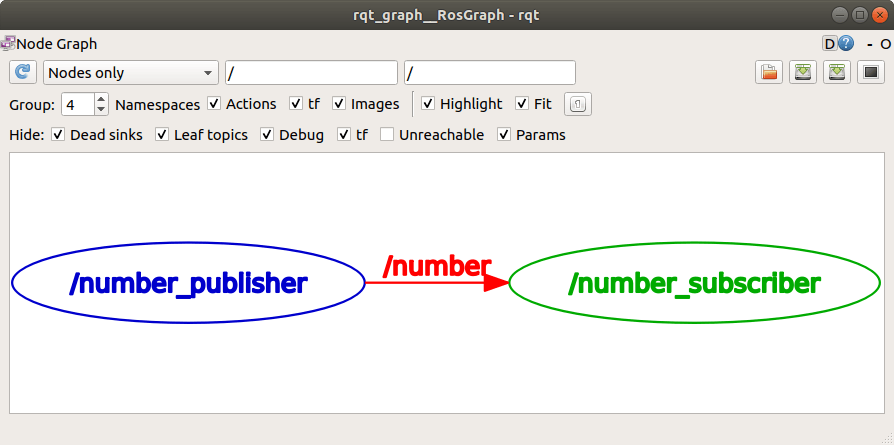
\includegraphics[height=5cm]{Bilder/rqt_graph_simplified.png}
			\caption{Ein vereinfachter Graph \\
			\parencite{rqtgraphsimplified1}} 
			\label{pic:rqt_graph_simplified}
		\end{figure}
	}

	\subsection{Drahtlose Übertragung}
	{ Wie bereits erwähnt, besitzt der Turtlebot einen Raspberry Pi. Dieser besitzt zwar für seine Größe vergleichsweise viel Leistung, jedoch wäre es natürlich vorteilhaft, die Rechenleistung eines herkömmlichen Desktop-PCs zu nutzen. Genau deshalb ermöglicht es das ROS, über mehrere Geräte hinweg zu kommunizieren. Das Herzstück bildet hierbei das ROS-Core Programm, welches alle Vorgänge innerhalb des Systems steuert. Dieses Programm muss auf einem der miteinander kommunizierenden Geräte aktiv sein. Mit Hilfe IP-Adressen \footnote{Ähnlich einer Adressanschrift: Zahlenkombination zur eindeutigen Identifikation eines Gerätes in einem Netzwerk} der Geräte kommunizieren die Teilnehmer untereinander in einem Netzwerk, als ob alle Pakete (Programme) auf einem Geräte ausgeführt werden würden. Dies ermöglicht das ausführen von Rechenintensiven Programmen auf einem Computer, während kleinere Programme, sowie der ROS-Core auf dem Turtlebot laufen. Das Gerät, auf welchem der Ros-Core läuft, wird auch ROS-Master genannt. Um beide Geräte zu verbinden, benötigt es nur wenige Einstellungen. Nachdem beide Geräte sich im gleichen Netzwerk befinden müssen die Parameter: \textbf{ROS\textunderscore IP} und \textbf{ROS\textunderscore Master \textunderscore URI} eingestellt werden. Ersterer beschreibt die IP-Adresse des Gerätes (für beide Geräte unterschiedlich) und letzterer Parameter beschreibt die IP-Adresse des ROS-Masters (für beide gleich, in meinem Fall ist es die Ip-Adresse des Turtlebot). Durch das ROS bauen beide Geräte eine Verbindung miteinander auf und kommunizieren miteinander.
	}
	
	\subsection{Simulation und Visualisierung}
	{
		Gazebo ist ein Open-Source-Programm \footnote{Frei zur Verfügung gestellt}, welches eine vollständige Simulation von Robotern, Umgebungen und Messungen ermöglicht. Robotermodelle können dazu modelliert werden, ebenso wie Umgebungen. Der Roboter kann sich daraufhin, wie in der realen Welt, bewegen und Messungen durchführen. Durch eine realistische Physik-Engine\footnote{Virtuelle Simulation physikalischer Kräfte} können Messungen wie in der echten Welt simuliert werden. D.h. der simulierte Roboter, in meinem Fall der Turtlebot, erhält Messdaten durch seinen Sensor, welche basierend auf der virtuellen Welt errechnet werden. Da ich einen größeren Teil meiner Arbeit von zuhause verrichtet habe, wurde dieses Programm oft genutzt, weshalb auch immer Bilder aus diesem Programm, anstelle von Bildern aus der echten Welt, gezeigt werden.
		
		Rviz ist ebenso ein Open-Source-Tool, welches es ermöglicht, Daten, ob gemessen oder errechnet, zu visualisieren. Dafür empfängt ROS Daten der Nodes und präsentiert diese auf geeigneter Weise. So kann beispielsweise die Momentane Bewegungsrichtung als Pfeil, Messdaten des LiDAR-Sensors als Punkte oder eine Errechnete Karte als Hintergrundbild angezeigt werden
		
		
	}
}
	%% !TEXroot=main.tex
\section{Turtlebot}
{
	\subsection{Überblick}
	{
		Der Turtlebot ist ein beliebtes Robotermodell der Firma Robotis und kommt in verschiedenen Varianten. Das gute Preis-Leistungs-Verhältnis, sowie die Einsteigerfreundlichkeit, kombiniert mit vielen Integration in andere Programme machen in zu einer guten Wahl für viele Projekte
		Der Turtlebot 3 besteht aus vier Basisplatten, auf welchen die gesamte Technik des Roboters untergebracht ist. Auf der untersten Basisplatte findet man zwei Servomotoren der X-Series von Dynamixel vor, welche dem Turtlebot seine Mobilität verleihen, auf den anderen Plattformen ist ein Raspberry PI 3, welcher unter Umständen auch durch einen Raspberry Pi 4 ersetzt werden kann, sowie ein Einplatinencomputer vorzufinden. Bei Letzterem handelt es sich standardmäßig um einen Intel Joule 570x. Auf der obersten Basisplatte findet man Platz für einen Sensor vor, dort kann eine Kamera, allerdings auch ein Lasersensor oder ähnliches angebracht werden. Auf unserem Turtlebot ist ein LiDAR-Sensor montiert. Dieser Sensor sendet Laserimpulse aus und kann durch das zurückgestrahlte Licht den Raum exakt vermessen. Der Roboter tastet die Umgebung mit den Laserimpulsen ab, was dazu führt, dass er Messpunkte erhält. 
		
		\begin{figure}[H]
			\centering
			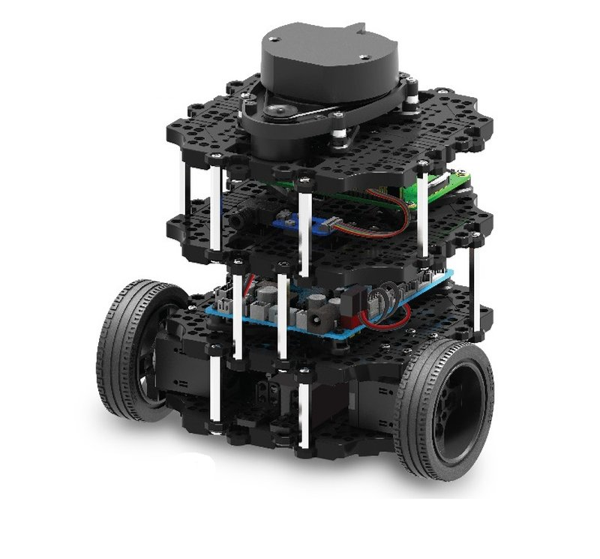
\includegraphics[height=5cm]{Bilder/turtlebot_3_burger.png}
			\caption{Der Turtlebot 3 in der „Burger“ Variante \\ \parencite{turtlebot3burger001}} 
			\label{pic:turtle3burger}
		\end{figure}
		
		%Diese Messpunkte kann der Roboter als Wände oder andere Formen interpretieren. Allerdings handelt es sich dabei um eine 2D Messung, welche in unserem Fall die Umgebung des Roboters auf Höhe des Sensors scannt. Der Sensor kann sich unabhängig vom Roboter um 360° drehen. Ein Problem des Roboters ist, dass er mit dem Standard Sensor keine Hindernisse erkennt, welche nicht auf der Höhe des Sensors sind. Rundum vereint der Roboter eine exzellente Leistung bei günstigen Preisen.
	}

	\subsection{LiDAR-Sensor}
	{
		Dieser Sensor sendet Laserimpulse aus und kann durch das zurückgestrahlte Licht den Raum exakt vermessen. Der Roboter tastet die Umgebung mit den Laserimpulsen ab, was dazu führt, dass er Messpunkte erhält. Diese Messpunkte kann der Roboter als Wände oder andere Formen interpretieren. Allerdings handelt es sich dabei um eine 2D Messung, welche in unserem Fall die Umgebung des Roboters auf Höhe des Sensors scannt. Der Sensor kann sich unabhängig vom Roboter um 360° drehen. 
		Die Distanz eines Punktes ergibt sich aus der Zeitdifferenz zwischen Aussendung und Empfangen einer elektromagnetischen Welle (Licht) im infraroten Bereich.
		Eine einfache Formel lautet wie folt:
		
		\begin{equation}
			s = c \cdot \frac{t}{2}
		\end{equation} 
		wobei $s$ die Entfernung, $t$ die Zeit zwischen Aussendung und Empfangen, sowie $c$ die Lichtgeschwindigkeit ist.
	
		Ein Problem für Roboters ist, dass mit Hilfe des Standard Sensor keine Hindernisse erkannt werden, welche nicht auf der Höhe des Sensors sind. Dies ist vor allem für Größere Roboter ein Problem, kann aber aufgrund der Umgebung des Roboters, sowie dessen Größen in der Labyrinth-Umgebung vernachlässigt werden.
		\begin{figure}
			\centering
			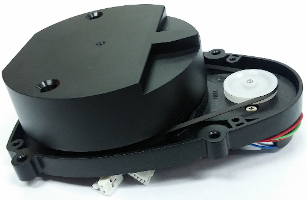
\includegraphics[height=5cm]{Bilder/lds_small.png}
			\caption{Der im Turtlebot 3 verbaute LiDAR-Sensor}
			\label{pic:lds_small}
		\end{figure}
	}
	
	\subsection{Raspberrry Pi}
	{
		Auf dem Turtlebot ist ein kleiner Computer, ein der Marke "Raspberry Pi" eingebaut. Standardmäßig handelt es sich dabei um das Modell der Reihe 3, welches jedoch aus Leistungsgründen mit einem Modell der 4. Generation ausgetauscht worden ist. Dieser Mikrocomputer stellt das Herzstück des Roboters dar und steuert alle Vorgänge. Wie ein jeder Computer besteht auch der Raspberry Pi aus einem Prozessor, Arbeitsspeicher, einer SD-Karte als Festplattenersatz und vielem mehr. Zwar stellt die Firma Raspberry auch eine graphische Benutzeroberfläche bereit, jedoch ist diese zur Programmierung nicht zweckführend, da diese Leistung verbraucht, welche für Berechnungen verwendet werden könnte. Aus diesem Grund verwende ich den Raspberry Pi mit einem einfachen Betriebssystem, welches nur eine Konsole anzeigt, um Leistung zu sparen.
	}
}
	%% !TEXroot=main.tex
\section{SLAM}
{
	\subsection{Überblick}
	{
		SLAM (\textit{Simultaneous Localization and Mapping, dt.: Simultane Positionsbestimmung und Kartierung}) beschreibt den Prozess, in welchem eine Karte durch Messdaten erstellt wird, wobei der Roboter selbst auf der Karte verordnet wird.
		Im Fall des Turtlebot geschieht dies mithilfe der Messdaten des LiDAR-Sensors, welcher die Entfernung von Objekten durch Laserstrahlen misst (\textit{siehe LiDAR-Sensor})	
	}

	\subsection{Positionierung}
	{
		Der Roboter wird anfangs auf den Mittelpunkt der, zu Beginn noch nicht vorhandenen Karte, welche erst durch Messdaten entsteht, platziert. Die Position des Roboters wird entsprechend der Bewegung seiner Motoren kalkuliert. Mithilfe des Umfangs der Reifen kann die bewegte Distanz errechnet werden, da dem Roboter die Winkeländerung der Motoren, z.B. eine Drehung dieser um 180°, bekannt ist. Diese werden an die Motoren übermittelt, wobei die Information noch an andere Teile weitergeleitet werden kann, hier der Microchip auf der Hauptplatine des Raspberry Pi 3 in der Mitte der Roboters, welcher damit Rechnungen, eben zur Positionskorrektur durchführen kann. Vereinfacht gilt daher bei einer geraden Bewegung
		\begin{equation}
			D = R \cdot U
		\end{equation} 
		
		Hierbei steht $D$ für die zurückgelegte Distanz, $R$ für die Umdrehungen der Motoren und $U$ für den Umfang der Reifen. Die Rotation, also die Drehung des Roboters, wird aus der Rotationsdifferenz beider Motoren berechnet. Dreht sich der rechte Motor weiter (größerer Winkel), so dreht sich der Roboter nach links, für eine Rechtsdrehung gilt das Gegenteil.
		Auf diese Weise kann nur aus den Daten, welche an der Motoren gesendet wird, errechnet werden wie weit und in welche Richtung der Roboter sich bewegt hat.
		Die benötigten Daten werden aus Odometrie-Daten gelesen. Dies sind interne Daten des Roboters, welche durch Messungen oder (wie oben genannt) Rechnungen erhält. Diese weichen durch Umwelteinflüsse und Messungenauigkeiten leicht von der Realität ab.
		
		
	}

	\subsection{Kartierung}
	{
		Die Kartierung erfolgt mithilfe der durch den LiDAR-Sensor gemessenen Daten. Dieser misst den Abstand des Roboters in verschiedene Richtungen punktartig. \newline  
		\begin{figure}[H]
			\begin{minipage}{0.5\textwidth}
				\centering
				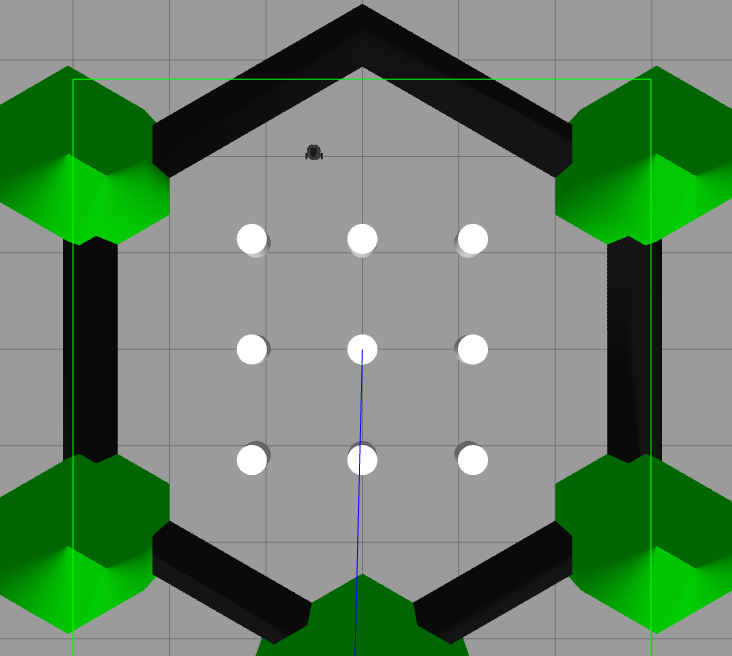
\includegraphics[height=5cm]{Bilder/virtualmap_world_gazebo.png}
				\caption{Roboter (zentriert im oberen \\ Drittel) in einer virtuellen \\Umgebung} %\parencite{flora85}}
				\label{pic:virtworldgazebo}
			\end{minipage}
			\begin{minipage}{0.5\textwidth}
				\centering
				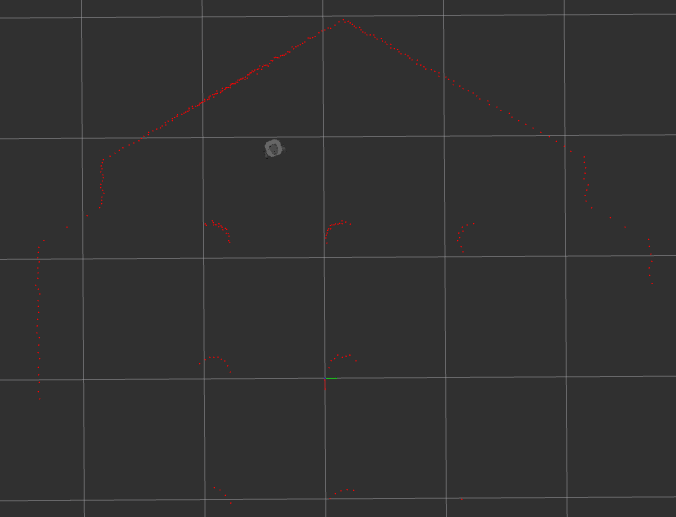
\includegraphics[height=5cm]{Bilder/virtualmap_world_rviz.png}
				\caption{Momentaufnahme der des LiDAR-Sensors gemessenen Punkte (Rot)}
				\label{pic:virtworldlaserrviz}	
			\end{minipage}
		\end{figure}
	
		Links erkennt man eine mit Gazebo simulierte Welt, in welcher sich der Roboter befindet, wobei er von Objekten (Säulen, Mauern) umgeben ist. Das rechte Bild ist ein Ausschnitt aus dem vorher erwähnte Programm Rviz, welches die durch den LiDAR-Sensor gemessene Punkte rot darstellt. Es ist zu erkennen, dass das Verbinden der Roten Punkte auf die Ursprüngliche Umgebung schließen lässt. Je näher der Roboter an einem Objekt ist, desto mehr Punkte befinden sich an dessen Stelle
		
		Zwar gibt eine Messung von einem Standpunkt einen akzeptablen Überblick, so werden jedoch viele Messungen von verschiedenen Stellen benötigt. Durch die Positionsänderung (\textit{siehe Positionierung}) kann errechnet werden wo neue Messpunkte im Vergleich zu alten Messpunkten liegen. Diese Positionierung der Punkte relativ zueinander wird schlussendlich zu einer Karte, wobei viele Messungen nötig sind. Da die Karte jedoch nur aus Punkten besteht, muss der Roboter diese noch interpretieren, sodass viele linear angeordnete Punkte z.B. als Wand interpretiert werden.
		
		Um eine komplette Karte zu erhalten Bewegt sich der Roboter durch die ihm noch unbekannte Welt, bis er eine Region durch genug Messpunkte Kartographiert hat und sich nun in Richtung einer ihm unbekannteren Region bewegen kann. Da der Roboter durch den LiDAR-Sensor konstant seine Umgebung misst, kann die Karte konstant verändert werden, vor allem, wenn der Roboter sich in Richtung weniger erforschte Gebiete bewegt.
		
		Während des Anfangs des Projektes wurde der Roboter noch mit Hilfe der Tastatur an einem Rechner oder über einen Logitech-Controller Gesteuert. Danach wurde daraus jedoch eine autonome Navigation, meist in Richtung von Gebieten, welche weniger erforscht sind. 
		
		Die Kartierung erfolgt mit Hilfe des \textit{gmapping}-Algorithmus. Dieser schaut sich die gescannten Laserdaten der \textit{sensor\textunderscore msgs/LaserScan}-Topic an und veröffentlicht drei Datenarten.
		\begin{enumerate}
			\item ein "Occupancy-Grid": 2D-Karte. Jeder Ort (Pixel) hat einen Ja/Nein Wert, welcher beschreibt, ob sich an der Position ein Objekt befindet oder nicht
			\item Entropie (Sicherheit über die Erkenntnis verschiedener Punkte: unsichere Punkte werden wahrscheinlicher geändert)
			\item Metadaten über die Karte.
		\end{enumerate}
	
		Durch die Kartierung dieses Algorithmus wird aus den einzelnen Laserscan-Daten nun eine Karte. Dies wird in den unteren Abbildungen dargestellt. Hierbei handelt es sich um die Karterung der in Abbildung 4 gezeigten Umgebung. Schwarze Punkte wurden als Hindernis erkannt, graue Stellen sind hindernisfreie Punkte. Die durch den LiDAR-Sensor gemessenen Punkte werden in grüner Farbe über die Karte gelegt. In Abbildung 7 und 8 ist zu erkenne, dass SChwarze Punkte nicht direkt mit Gemessenen Punkten des Lasers (grün) übereinstimmen. Dies liegt zum einen darin, dass die Berechnung der Karte Zeit benötigt, weshalb die Punkte noch verarbeitet werden, sowie daran, dass die Aktualisierungsrate der Karte eingestellt werden kann. Während intuitiv eine schnelle Aktualisierungsrate sinnvoll wirkt, ist eine zu schnelle Rate nachteilig, da viel Leistung benötigt wird und mehr Fehler gemacht werden, da ungenaue Messpunkte zu schnellen Schlüssen auf der Karte führen. Bei einer längeren Zeitdauer zwischen Kartenaktualisierungen können nämlich mehr gemessene Punkte in Betracht gemessen werden.
		
		\begin{figure}[H]
			\begin{minipage}{0.5\textwidth}
				\centering
				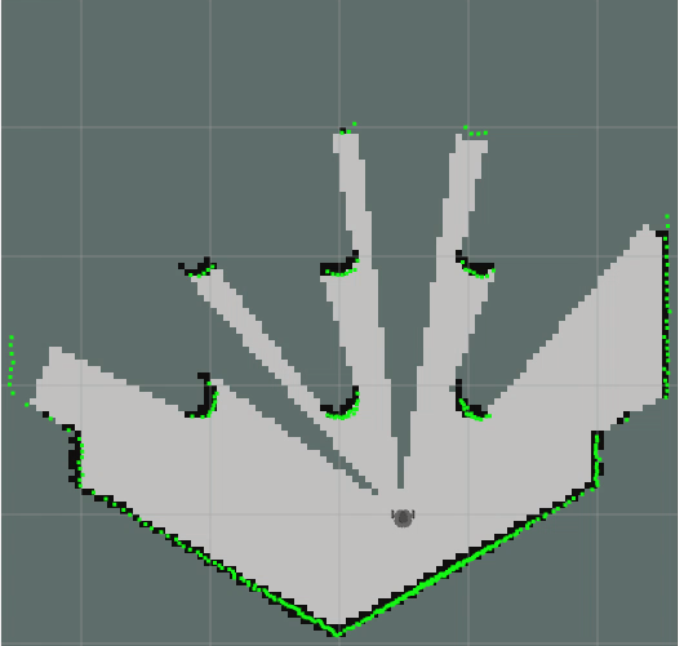
\includegraphics[height=5cm]{Bilder/mapping_smpl_1.png}
				\caption{Kartierung am Anfangspunkt}
				\label{pic:mapping_smpl_1}
			\end{minipage}
			\begin{minipage}{0.5\textwidth}
				\centering
				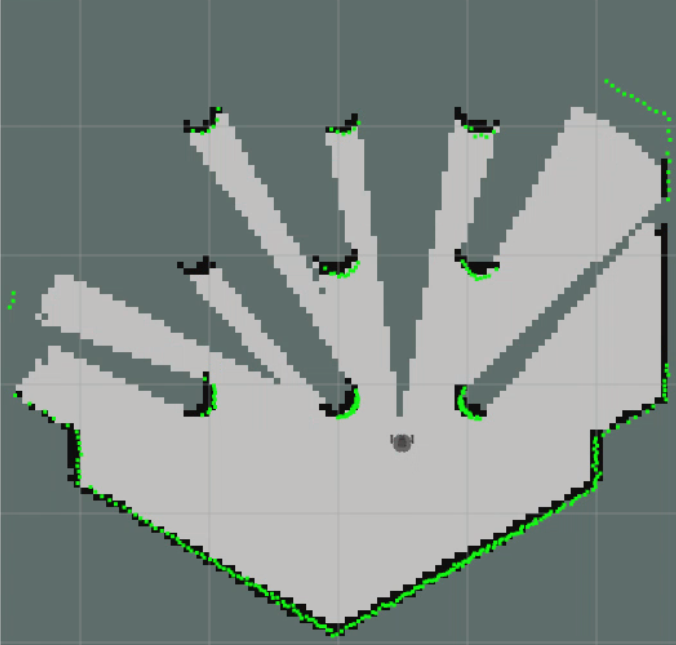
\includegraphics[height=5cm]{Bilder/mapping_smpl_2.png}
				\caption{Kartierung nach erster Bewegung (nach oben)}
				\label{pic:mapping_smpl_2}	
			\end{minipage}
		\end{figure}
		\begin{figure}[H]
			\begin{minipage}{0.5\textwidth}
				\centering
				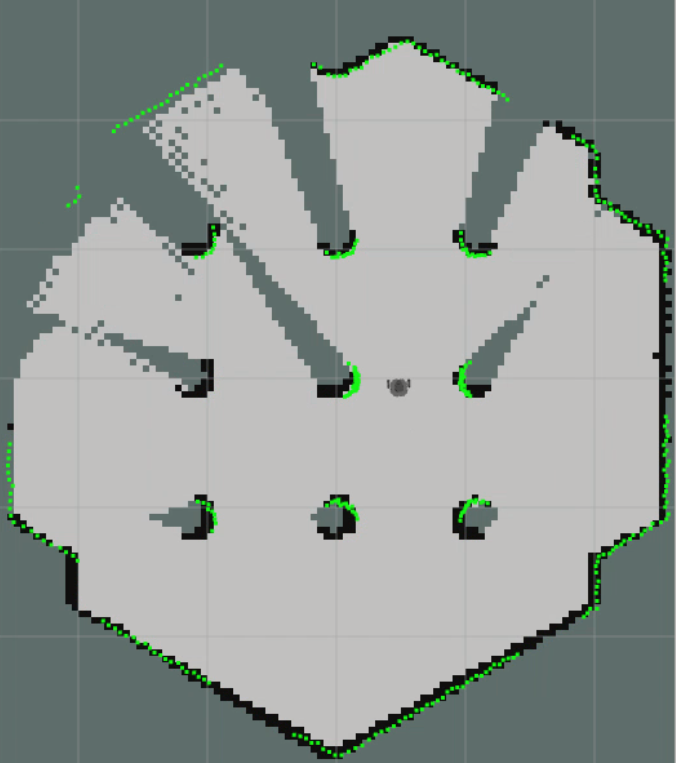
\includegraphics[height=5cm]{Bilder/mapping_smpl_3.png}
				\caption{Kartierung nach weiterer Bewegung}
				\label{pic:mapping_smpl_3}
			\end{minipage}
			\begin{minipage}{0.5\textwidth}
				\centering
				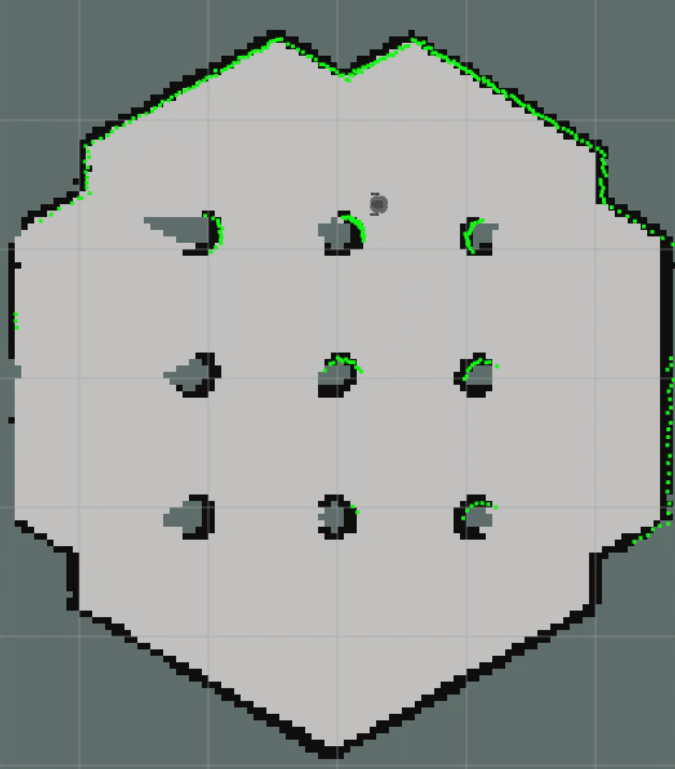
\includegraphics[height=5cm]{Bilder/mapping_smpl_4.png}
				\caption{Kartierung nach Erreichen des oberen Endes}
				\label{pic:mapping_smpl_4}	
			\end{minipage}
		\end{figure}
	}
}
	%% !TEXroot=main.tex
\section{Pathfinding}
{
	\subsection{Definition}
	{
		Pathfinding (\textit{engl. Wegfindung}) beschreibt den Prozess der Wegfindung, wobei der kürzestmöglichen Weg von einem Startpunkt zu einem Zielpunkt gefunden werden soll. Dieser Prozess setzt eine Karte der Umgebung (\textit{siehe SLAM}), in welcher ein Weg gefunden werden soll, voraus.
	}

	\subsection{Anwendung in der heutigen Welt}
	{
		Pathfinding-Prozesse sind von heutiger Technologie nicht mehr zu trennen. Sie sind überall präsent und helfen uns, auch wenn wir es manchmal nicht bemerken . Navigationssysteme müssen die kürzeste Route zu einem Zielpunkt finden, wohingegen Staubsaugroboter Orte in einem Haus erreichen müssen. Signale über Satelliten hinweg werden auch über den kürzesten Weg geleitet. Diesen zu finden bedeutet immer, dass für den Transport weniger Aufwand und Zeit benötigt wird
	}

	\subsection{Algorithmen zur Umsetzung}
	{
		Für die Wegfindung gibt es viele etablierte Algorithmen, jedoch stellt sich nun die Frage, welcher am Nützlichsten ist. Diese Nützlichkeit wird meist an zwei Faktoren gemessen. Diese sind zum einem die Genauigkeit, welche beschreibt ob ein Algorithmus den besten Weg findet, und zum anderen die Geschwindigkeit. Diese beschreibt, wie effizient ein Algorithmus den idealen Weg findet. Mit Geschwindigkeit ist also nicht die Zeit der Ausführung gemeint, welche mit der Effizienz jedoch stark zusammenhängt, da diese je nach genutzten Bauteilen in Computern variiert. Vielmehr wird, wie erwähnt, die Rechenintensität als Maß genutzt. Diese beschreibt, wie viele Schritte durchgeführt werden müssen, bis der ideale Weg gefunden wurde. Je geringer, desto besser. 
		
		Viele Wegfindungsalgorithmen nutzen das gleiche Grundprinzip. Die Karte wird in kleine Vierecke unterteilt. Vom Startpunkt aus wird nun in eine Richtung gegangen und zwar einen Schritt weit. Dabei wird diese Stelle als "besucht" angesehen, wobei von ihr aus nun in weitere Richtungen gelaufen werden kann (Abbildung \ref{pic:pathfinding_procedure_1}). Grenzt eine besuchte Fläche an das Ziel an, so wurde ein Weg gefunden. Nachdem anfangs in jede Richtung ein Schritt in die Tiefe gegangen wurde, wird nun erneut in eine andere Richtung gegangen, bis in jede Richtung ein Schritt gegangen bzw. abgesucht worden ist (Abbildung \ref{pic:pathfinding_procedure_4}). Eine Tiefe (Längeneinheit) wurde somit vollständig abgedeckt. Daraufhin wird nun das Gleiche mit einer Tiefe von zwei zum Startpunkt hin wiederholt wird.
		
		\begin{figure}[H]
			\begin{minipage}{0.5\textwidth}
				\centering
				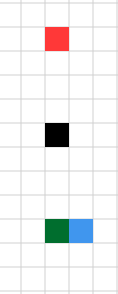
\includegraphics[height=5cm]{Bilder/pathfinding_procedure_1.png}
				\caption{\\ 1. Feld wird durchlaufen} 
				\label{pic:pathfinding_procedure_1}
			\end{minipage}
			\begin{minipage}{0.5\textwidth}
				\centering
				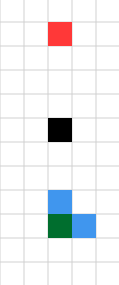
\includegraphics[height=5cm]{Bilder/pathfinding_procedure_2.png}
				\caption{\\ 2. Feld wird durchlaufen} 
				\label{pic:pathfinding_procedure_2}
			\end{minipage}
		\newline
			\begin{minipage}{0.5\textwidth}
				\centering
				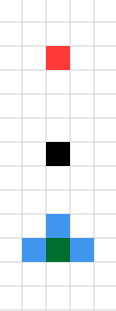
\includegraphics[height=5cm]{Bilder/pathfinding_procedure_3.png}
				\caption{\\ 3. Feld wird durchlaufen} 
				\label{pic:pathfinding_procedure_3}
			\end{minipage}
			\begin{minipage}{0.5\textwidth}
				\centering
				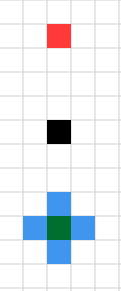
\includegraphics[height=5cm]{Bilder/pathfinding_procedure_4.png}
				\caption{\\ 4. Feld wird durchlaufen}
				\label{pic:pathfinding_procedure_4}
			\end{minipage}
		\end{figure}
		
		
		%evtl \newpage
		Dies wird in der unteren Abbildung verdeutlicht. Grün repräsentiert den Startpunkt, Rot den Endpunkt. Schwarz repräsentiert ein nicht passierbares Feld und blaue Felder sind von dem Suchalgorithmus bereits besucht worden. 
		Die dargestellte Suchart stellt den \textbf{Breadth-first Search Algorithmus} dar, welche zur oben gegebenen Beschreibung passt. Dabei handelt es sich um einen einfachen Wegfindungsalgorithmus.
		
		\begin{figure}[H]
			\begin{minipage}{0.5\textwidth}
				\centering
				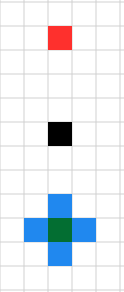
\includegraphics[height=5cm]{Bilder/pathfinding_tiefe1.png}
				\caption{Besuchte Felder nachdem die \\ Tiefe 1 durchlaufen wurde} %\parencite{flora85}}
				\label{pic:pathtiefe1}
			\end{minipage}
			\begin{minipage}{0.5\textwidth}
				\centering
				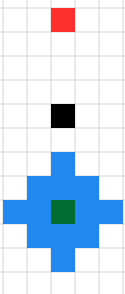
\includegraphics[height=5cm]{Bilder/pathfinding_tiefe2.png}
				\caption{Besuchte Felder nachdem die \\ Tiefe 2 durchlaufen wurde} %\parencite{northFlora190105}}
				\label{pic:pathtiefe2}
			\end{minipage}
		\end{figure}	
	
		Zur Verbesserung der Effizienz nutzen manche Algorithmen weitere Algorithmen, die Schätzalgorithmen, welche man auch Heuristik nennt, die Einfluss darauf nehmen, welche Felder als nächstes besucht werden. Felder, welche in Richtung des Ziels zeigen bzw. sehr wahrscheinlich dorthin führen, werden bevorzugt durchlaufen, Felder, welche vom Ziel weg zeigen, werden hingegen seltener Besucht. Dazu misst der Algorithmus nicht nur die Distanz(Kosten) bis zu einem Punkt, um zu berechnen, ob es sich lohnt, von diesem aus weiter zu suchen, sondern auch die Distanz zum Ziel. Mathematisch kann man dies als zusammengesetzte Funktion verstehen.
		\begin{equation}
			f(x) = g(x) + h(x)
		\end{equation}
		
		Hierbei stellt $g(x)$ die Funktion dar, welche die Kosten(Distanz) vom Startpunkt bis zu einem Punkt $x$ berechnet. $h(x)$ beschreibt die vermutete Distanz von $x$ bis zum Zielpunkt. Beide Ergebnisse zusammen ergeben einen Wert, welcher die Kosten über einen Punkt $x$ zum Zielpunkt errechnet. Dies wird für viele Punkte $x$ berechnet, wobei der nächste Schritt von dem Punkt ausgeht, welcher den niedrigsten Wert (also die geringste, errechnete Distanz) hat.
		Diese Algorithmen sind für viele Verwendungszwecke sehr effizient. Heuristik nutzende Wegfindungsalgorithmen können unter Umständen nachteilig sein, wenn diese in Labyrinthen eingesetzt werden, welche eine hohe Komplexität aufweisen, da Sackgassen, welche nur durch eine Wand vom Ziel getrennt werden, meist durchsucht werden, obwohl sie im Endeffekt nicht Zielführend sind.
		
		\begin{figure}[H]
			\centering
			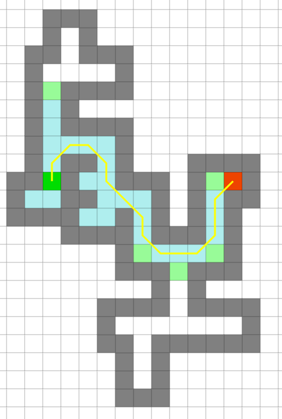
\includegraphics[height=5cm]{Bilder/pathfinding_laby_heu.png}
			\caption{Wegfindung eines Algorithmus mit Heuristik} 
			\label{pic:pathlabheu}
		\end{figure}
		
		\subsection{Coastmap}
		{
			Eine gemessene Karte wird zur Navigation zu einer Coastmap umgewandelt. Diese enthält Daten, welche während  der Kartenerstellung nicht angezeigt, trotzdem aber gesammelt werden. Im Falle einer Coastmap wird nicht nur betrachtet, ob ein Punkt besetzt oder frei ist, sondern auch, wie schwierig es ist, gewisses Terrain zu überqueren. Zwar sind diese Daten in einer ebenen Fläche relativ irrelevant, vor allem aber bei hügeligem Boden sind diese interessanter, weshalb ich dies hier erwähnen wollte. Dies weiteren erhalten Hindernisse einen Radius, welcher von dem Roboter tendenziell vermieden werden sollte, da Kollisionen, u.a. aufgrund der Objektform oder ungenauer Messdaten möglich sein Könnte.
		}
		
		\subsection{Positionierung auf einer Karte}
		{
			Zwar hat der Roboter nun eine Karte seiner Umgebung, jedoch fehlt dem Roboter noch sein genauer Standpunkt, da er sich auf irgendeinem Punkt in der Karte befinden könnte. Um nun den genauen Standpunkt zu finden, nutzt man die Monte-Carlo-Lokalisation. Dafür wird die Karte der Umgebung, sowie die Sensordaten, benötigt. Anfangs ist es gleich wahrscheinlich, dass der Roboter sich in jeglicher Stelle auf der Karte befindet. Nun werden die gemessenen Sensorpunkte und die Karte der Umgebung übereinander gelegt. Stimmen Hindernisse, welche durch die Karte in der Nähe sind, sowie gemessene Sensordaten der realen Welt überein, so ist es wahrscheinlich, dass sich der Roboter an dieser Stelle in der Karte befindet. Misst der Turtlebot beispielsweise einen Runden Gegenstand vor sich und in einer Position auf der Karte ist in gleicher Distanz eine Runde Säule vor dem Roboter, so ist es wahrscheinlich, dass der Roboter sich in dieser Position befindet. In der beigefügten Abbildung, wird das vergleichen von Sensordaten und Karte deutlich.
			\begin{figure}[H]
				\centering
				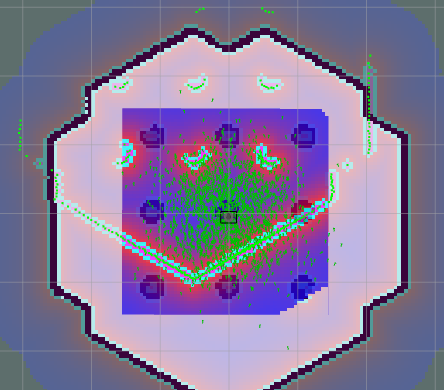
\includegraphics[height=5cm]{Bilder/coastmap_monte_carlo_example.png}
				\caption{Coastmap mit Sensordaten} 
				\label{pic:coastmontecarlo}
			\end{figure}
		In der Abbildung wird deutlich, dass der Roboter auf der gegebenen Karte (Hintergrund) mittig platziert wird. Gleichzeitig misst der LiDAR-Sensor auch Hindernisse, welche wiederum eine neue Karte der Umgebung bilden. Diese Hindernisse sind Hell im Vordergrund zu sehen. Man erkennt, dass diese nicht übereinander liegen und der Roboter deshalb noch nicht korrekt positioniert ist. In Wirklichkeit werden Daten aus der unteren linken Ecke der Karte gemessen. Dadurch werden Positionen in dieser Umgebung sehr wahrscheinlich. Damit der Roboter bei vielen ähnlichen Stellen, was hier nicht der Fall ist, trotzdem korrekt positioniert ist, wird der Roboter zwischen verschiedenen LiDAR-Messungen bewegt. Während der Bewegungen wird errechnet, wo der Roboter sich, ausgehend von den Ursprünglichen Vermutungen der Position, befindet. Stimmen auch die neuen Messungen mit der Karte überein, so wird eine Position immer wahrscheinlich, bis der Roboter schlussendlich, sicher positioniert werden kann, da Sensordaten und Karte übereinstimmen. im Falle anderer Roboter können neben LiDAR-Sensoren auch andere Sensordaten verwendet werden.
		}
		\subsection{Die Move-Base} %https://www.researchgate.net/publication/253239158_ROSoClingo_A_ROS_package_for_ASP-based_robot_control
		{
			Um den Roboter nun zu einem Ziel zu navigieren, wird das move\textunderscore base-Package verwendet. Dieses steuert die Navigation des Roboters, sowie den Pfad, welchem der Roboter folgen soll. Es besteht aus mehreren Nodes (in der Abbildung oval dargestellt).  Dazu abonniert diese Nodes verschiedene Topics. Dazu gehören Sensordaten (z.B. sensor\textunderscore msgs/LaserScan für die Daten des LiDAR-Sensors), Odometriedaten und eine Karte. Die Karte wird durch einen Kartenserver bereitgestellt, welcher, als Node, diese Karte veröffentlicht, sodass jegliche Programme darauf zugreifen können. Dafür muss die Karte jedoch als Bild vorliegen, weshalb die Karte nach vollendeter Kartierung des Labyrinth auf einem Datenträger, meist die Festplatte eines über Wifi mit dem Turtlebot verbundenen Computers, gespeichert werden muss. Die gespeicherte Karte kann daraufhin von dem Karten-Server geöffnet werden. Dieses System sorgt gleichzeitig dafür, dass man eine Umgebung zur Navigation nicht notwendigerweise erneut kartieren muss, sollte schon eine Karte existieren. Im Anwendungsfall ist dies auch praktisch. Staubsageroboter müssen daher beispielsweise nicht jedes mal erneut eine komplette Karte eines Hauses erstellen.
		\begin{figure}[H]
			\centering
			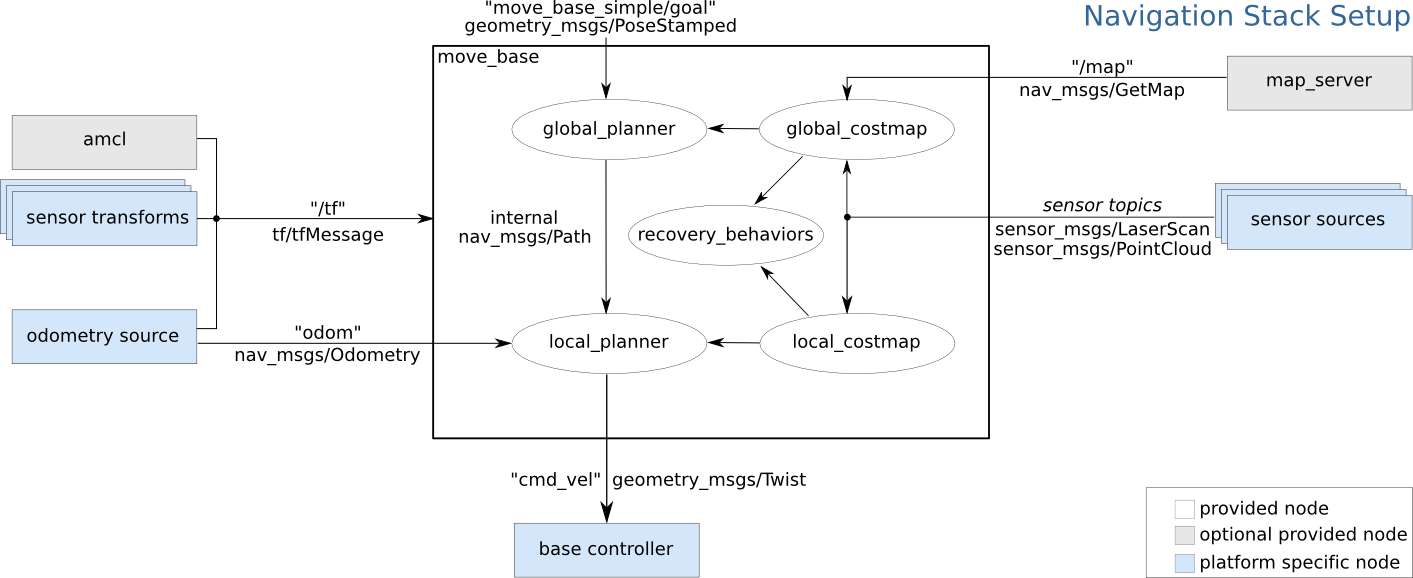
\includegraphics[height=8cm]{Bilder/overview_move_base.png}
			\caption{Das move\textunderscore base-Package \\
			\parencite{movebasenodeoverview}} 
			\label{pic:overviewmovebase}
		\end{figure}
			
			 Nachdem der Roboter nun auf der durch den Kartenserver bereitgestellten Karte verordnet ist, muss dem Roboter ein Navigationsziel gegeben werden.
			 Dazu gibt es mehrere Möglichkeiten. Das Programm Rviz ermöglicht es, wie bereits erwähnt, die Karte zu visualisieren. Gleichzeitig hat dies den Nebeneffekt, dass man durch das Programm bestimmen kann, welche Koordinaten ein Punkt auf der Karte hat, indem man die Maus auf diesen Bewegt. Rviz ermöglicht es sogar, direkt im Programm ein Navigationsziel festzulegen, was jedoch teilweise von dem Roboter nicht akzeptiert wird, weshalb ich ein Skript nutze, um die Koordinaten des Zielpunktes, welche ich in Rviz ablesen kann, an das move\textunderscore base-Package zu übertragen.
			 Dafür wird folgendes Skript verwendet, in welchem der Roboter sich beispielhaft zu dem Punkt $P(3|2)$ bewegen soll:
			 \newline  %https://answers.ros.org/question/80646/python-sending-goals-to-the-navigation-stack/
			
			\lstset{
				breaklines = true,
				frame = single,
				numbers = none
			}
\begin{lstlisting} [language=Python]
	01 import actionlib
	02 import rospy
	03 from move_base_msgs.msg import MoveBaseAction, MoveBaseGoal,   MoveBaseFeedback, MoveBaseResult
			 	
	04 rospy.init_node("nav_goal_sender")
			 	
	05 client = actionlib.SimpleActionClient("/move_base", MoveBaseAction)
	06 client.wait_for_server()
			 	
	07 goal = MoveBaseGoal()
	08 goal.target_pose.header.frame_id = 'map' 
	09 goal.target_pose.pose.position.x = 3
	10 goal.target_pose.pose.position.y = 2
	11 goal.target_pose.pose.orientation.z = 0
	12 goal.target_pose.pose.orientation.w = 0.5
			 	
	13 client.send_goal(goal)
	14 client.wait_for_result()
			 	
\end{lstlisting}
		 	Nun erläutere ich das Programm kurz Stück für Stück.
		 	Mit Hilfe der \textbf{import}-Befehle werden Bibliotheken eingebunden (Z. 1-3), welche Funktionalitäten für das Programm beinhalten, welche benötigt werden. Dazu zählt z.B: \textbf{rospy} (Z.2), welches eine Interaktion mit dem ROS-Betriebssystem ermöglicht, sowie verschiedene Klassen  \footcite{Programmierung: Ansammmlung von Funktionen (eines Aufgabenbereiches)}, welche mit dem move\textunderscore base-Package zusammenhängen (Z.3).
		 	
		 	Daraufhin wird eine Node-initiiert, deren einzige Funktion ist, ein Navigatinsziel auszusenden. Die Node erhält den Namen "\textit{nav\textunderscore goal\textunderscore sender}" (Z.4).
		 	
		 	In den nächsten zwei Zeilen wird ein "Action-Client" \space initiiert. Dies ist eine Klasse, welche es ermöglicht, eine Action an einen Service auszusenden. Diese Art des Datenaustausches wurde in Abschnitt 1.3.2- "Services" ausgeführt. Die Initiierung bedeutet vereinfacht gesagt, dass alles vorbereitet wird, sodass ein Befehl an den Service des move\textunderscore base-Packetes gesendet werden kann (Z.5f.).
		 	
		 	In den nachfolgenden sechs Zeilen (Z.7-12) werden die Parameter gesetzt, welche die Position, zu welcher Navigiert werden soll, bestimmen. Hier ist die z-Koordinate irrelevant, da der Roboter sich nicht nach oben/unten bewegen kann. Die x Koordinate (Z.9) wird gleich drei gesetzt. Die y-Koordinate gleich 2 (Z.10). In Zeile 11 wird die Richtung, in welche der Roboter am Ende schauen soll, festgesetzt.
		 	
		 	In Zeile 13 wird eine Action, also der Befehl mit den eingestellten Parametern, hier sind dies die Koordinaten, an den move\textunderscore base Service geschickt, welcher daraufhin zu diesem Ziel navigiert.
		 	
		 	
			
		}
	}
}
	
	% !TEXroot=main.tex
\section{Einleitung}
{
	Für uns Menschen ist das orientieren eine alltägliche Aufgabe. Ob in der Stadt, auf dem Weg nach Hause oder in einem Bürogebäude. Roboter, welche immer mehr Aufgaben automatisieren, haben das gleiche Problem. Auch diese müssen sich in Umgebungen zurechtfinden. Von Staubsaugrobotern zu autonom fahrenden Fahrzeugen, all diese Systeme müssen sich in einer verzweigten Umgebung zurechtfinden. Daher ist es auch in Wettbewerben beliebt, Aufgaben zu diesem Thema zu stellen. So auch im "`RoboCup" \copyright. Roboter müssen sich in einem Labyrinth zurechtfinden und verschiedene Aufgaben bewältigen. Daher kommt auch die Id\texttt{}ee für dieses Projekt. Ein Roboter soll sich in einem Labyrinth zurechtfinden - mit Hilfe einer selbst erstellten Karte. Basierend auf einer vereinfachten Version des ``RoboCup Rescue Maze`` ist das Ziel des Projekts die autonome Navigation, wobei jedoch keine Aufgaben wie beispielsweise die Rettung von Personen erfüllt werden. Dies geschieht basierend auf einem Turtlebot-Roboter, auf welchem das Robot-Operating-System operiert. Ziel ist, einen Roboter zu bauen, welcher in einem komplexen Labyrinth werden kann, welches auch Zyklen besitzt und somit nicht durch das Folgen einer Wand vollends durchlaufen werden kann.
}
	% !TEXroot=main.tex

\section{Grundlagen}
{
	\subsection{ROS}
	{
		\subsubsection{Überblick}
		{
			Das sogenannte Robot Operating System, kurz ROS genannt, ist ein Open-Source Betriebssystem für Roboter, welches viele Tools und Software-Bibliotheken bietet. Die Entwicklung von ROS begann 2007 im Stanford Artificial Intelligence Laboratory. Ab 2009 wurde ROS im Institut Willow Garage fortgeführt, bis ROS ab 2012 von der OSRF (Open Source Robotic Foundation) unterstützt wird. Seit der Veröffentlichung von ROS gibt es regelmäßig Updates und neuere Versionen von ROS, welche hauptsächlich mit Betriebssystem Linux, aber auch Windows oder MacOS kompatibel sind. 
			
			Die grundsätzliche Idee von ROS ist, alle Vorteile von vergleichbaren Produkten zu vereinen, während die Nachteile der jeweiligen Produkte behoben werden. Die Hauptbestandteile von ROS sind: Hardwareabstraktion, Gerätetreiber, Nachrichtenaustausch zwischen Programmen und Programmteilen und die Paketverwaltung. Alle diese Bestandteile sorgen dafür, dass der Roboter einfacher auf Daten zugreifen kann. Es handelt sich dabei um den aktuellen internationalen Standard, welcher auf den meisten Systemen einwandfrei läuft und dabei wenig Leistung beansprucht. Ein Gerätetreiber ist ein Programm, welches die Interaktion mit angeschlossenen, eingebauten oder virtuellen Geräten steuert. Beim Nachrichtenaustausch werden Nachrichten zum Empfänger versendet, bei welchen es sich um Signale oder Datenpakete handeln kann. Die Paketverwaltung hilft bei der Verwaltung von Software, die in Form von Programmpaketen vorliegt. Ein weiteres Ziel von ROS ist, oft wiederverwendbare Funktionen zugänglich zu machen. 
			
		}
		
		\subsubsection{Aufbau}
		{ Programme werden in ROS als Pakete implementiert. Ein Paket besteht aus einer Manifestdatei, welche Metadaten (z.B. den Autor) über das Paket beinhaltet, sowie ausführbaren Skripten (Programmen). Pakete werden meist unabhängig voneinander entwickelt, können doch miteinander kommunizieren (siehe Datenaustausch). Pakete können (ähnlich zu Apps auf einem Handy) einzeln installiert bzw. deinstalliert werden, wobei einige Pakete andere benötigen, um zu funktionieren. Die Programme werden meist in den Programmiersprachen C++ oder Python geschrieben, welche beide die größte Integration in das ROS vorweisen.
			
			Der ROS-Core ist der Mittelpunkt des Betriebssystems. Dieses Programm steuert alle Vorgänge und sorgt dafür, dass Daten an korrekte Pakete weitergegeben werden, sowie vieles mehr. 
			
			Eine Grundkomponente von ROS sind sogenannte Nodes (Knotenpunkte), welche von Programmen initiiert werden können: Jede dieser Nodes hat eine gewisse Funktion (z.B. das ansteuern von Motoren). Diese Punkte sind des Weiteren austauschbar, sodass es für verschiedene Motorenmodelle beispielsweise andere Nodes gibt, welche jedoch alle die gleiche Funktion erfüllen, nämlich das ansteuern der Motoren.
		}
	
		\subsubsection{Vorteile}
		{
			Der größte Vorteil des ROS ist die Aufteilung des Systems in universelle Komponenten. Der Datenaustausch der Komponenten ist standardisiert, \dahe die Daten, welche beispielsweise an Motoren weitergegeben werden, haben immer die gleiche Form. Dadurch können Hersteller für ihre Motoren Programme entwickeln, denn die Daten, welche an die Komponente zur Motorensteuerung weitergegeben werden. Gleiches gilt auch für die Ausgabe von Daten durch einzelne Komponenten. Diese Standardisierung von Daten erlaubt eine Flexibilität in der Spezifität der einzelnen Komponenten und erlaubt eine einfache Integration. Dadurch wird eine Kollaboration vieler Menschen überall auf der Welt ermöglicht. Forschungsergebnisse, wie \zb GMapping, worauf ich später eingehen werde, werden damit für jedermann verfügbar und können leicht in die eigenen Systeme eingebunden werden.
		}
		
		\subsubsection{Datenaustausch}
		{
			Der Austausch von Daten kann sich als Graph vorgestellt werden. Jeder Knotenpunkt kann Daten aussenden oder empfangen. Der Datentyp, welcher ausgetauscht wird, kann beliebig bestimmt werden, jedoch beruht alles auf vier Grundtypen.
			\begin{enumerate}
				\item Ganzzahlen (Integer)
				\item Kommazahlen (Float)
				\item Zeichen (Char)
				\item Ja/Nein (Boolean)
			\end{enumerate}
			Basierend auf diesen Grundtypen können neue Datentypen gebaut werden. So kann man beispielsweise sagen, dass der Datentyp Auto
			\begin{enumerate}
				\item eine Kommazahl hat, welche den Füllstand beschreibt,
				\item eine ganze Zahl hat, welche die Anzahl an Passagieren beschreibt,
				\item ein aus mehreren Zeichen bestehendes Kennzeichen hat,
				\item einen Ja/Nein-Wert hat, welcher bestimmt, ob der Motor an ist,
			\end{enumerate}
			
			hat. Die Datenstruktur der ausgetauschten Daten wird Nachricht genannt. Nodes tauschen also Nachrichten untereinander aus. Jede Nachricht bekommt eine sogenannte Topic, was die Nachricht und deren Struktur eindeutig identifiziert. Ein Beispiel hierfür ist die \textit{cmd\textunderscore vel} Topic, welche Nachrichten des Types \textit{geometry\textunderscore msgs/Twist} weitergibt. Diese Daten geben Informationen über die aktuelle Begungsrichtung wieder. Zur vereinfachung zeige ich nur die Richtungen der Bewegung im 3D-Raum, nicht aber der Drehung, da diese für das Verständnis nicht notwendig ist. Die Struktur der Nachricht sieht daher (in gekürzter Fassung folgendermaßen aus:
			\newline
			
			linear:
			\begin{itemize}
				\item float64 x
				\item float64 y
				\item float64 z
			\end{itemize}
			
			\textit{float64} stellt in der Programmierung eine Kommazahl dar. Daraus folgt, dass diese Nachricht drei Zahlen für jede Richtung hat, woraus sich die Bewegungsrichtung des Roboters ergibt. Im Falle meiner Navigation ist die z-Koordinate irrelevant, da der Roboter sich nicht nach oben/unten bewegt, sondern nur auf der 2 dimensionalen Ebene.
		}
		
		\subsubsection{Publisher-Subscriber}
		{
			Nodes sind von Programmen initiierte Knotenpunkte, auf welche das Programm ,welches sie initiiert hat, Zugriff hat. Über diese Punkte können Daten bereitgestellt werden, indem das Programm diese publiziert (Publisher). Dies kann man sich wie ein Forum darstellen, in welchem eine Person mit einem Megafon die Daten verkündet. Andere Nodes (Listener/Subscriber) können diesen Punkt nun abonnieren, was bedeutet, dass die Daten an sie weitergeleitet werden. Diese Listener-Nodes sind vergleichbar mit Personen, die das Forum betreten und daher alles hören, was der Redner (Publisher-Node) sagt. bei dieser Variante des Datenaustausches bestimmt der Publisher, wann Daten verbreitet werden. Mehrere Listener-Nodes können eine Publisher-Node abonnieren.
		}
		\subsubsection{Services}
		{ 
			Services bilden das Gegenstück zum Publisher-Subscriber-Modell. Hierbei stellt eine Node Aufgaben bereit, welche sie auf Anforderung erfüllt. Node A bietet beispielsweise an, die Lichter in einem Raum an bzw. auszuschalten. Node B kann in diesem Fall auf den Service "Ändere Lichtzustand" von Node A zugreifen, woraufhin Node A das Licht an bzw. ausschaltet. Ohne Aufruf führt Node A dies jedoch nicht durch. Dies zeigt, dass bei diesem Modell nicht, die Node, welche einen Service bereitstellt, den Zeitpunkt der Ausführung definiert, sondern ein anderer Punkt, welcher den Service aufruft.
		}
		
		\subsubsection{Visualisierung des Datenaustausches}
		{
			Der Datenaustausch zwischen verschiedenen Nodes kann mit Hilfe einfacher Tools visualisiert werden. Ein sehr wichtiges Tool ist \textit{rqt\textunderscore Graph}, welches alle Knoten und deren Zusammenhänge als Graphen anzeigt. Dabei werden Nodes als Punkte und deren Verbindungen als Linien angezeigt. Verbindungen werden mit dem Namen der Topic an Daten, die Übertrieben werden, beschriftet. Dies ist vereinfacht in Abbildung 1 dargestellt. Hierbei veröffentlicht die Node \textit{number\textunderscore publisher} Daten der Topic \textit{/number} an die Node \textit{number\textunderscore subscriber} (rechts), welche die linke Node abonniert hat.
			
			\begin{figure}
				\centering
				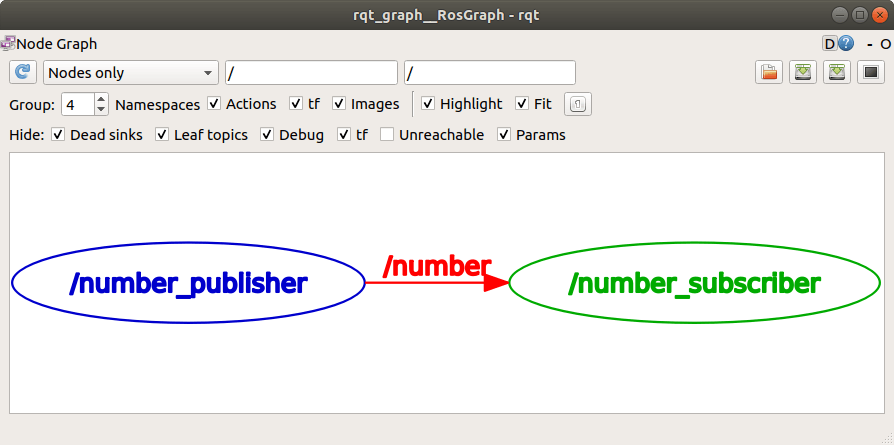
\includegraphics[height=5cm]{Bilder/rqt_graph_simplified.png}
				\caption{Ein vereinfachter Graph \\
					\parencite{rqtgraphsimplified1}} 
				\label{pic:rqt_graph_simplified}
			\end{figure}
		}
		
		\subsubsection{Drahtlose Übertragung}
		{ Wie bereits erwähnt, besitzt der Turtlebot einen Raspberry Pi. Dieser besitzt zwar für seine Größe vergleichsweise viel Leistung, jedoch wäre es natürlich vorteilhaft, die Rechenleistung eines herkömmlichen Desktop-PCs zu nutzen. Genau deshalb ermöglicht es das ROS, über mehrere Geräte hinweg zu kommunizieren. Das Herzstück bildet hierbei das ROS-Core Programm, welches alle Vorgänge innerhalb des Systems steuert. Dieses Programm muss auf einem der miteinander kommunizierenden Geräte aktiv sein. Mit Hilfe IP-Adressen \footnote{Ähnlich einer Adressanschrift: Zahlenkombination zur eindeutigen Identifikation eines Gerätes in einem Netzwerk} der Geräte kommunizieren die Teilnehmer untereinander in einem Netzwerk, als ob alle Pakete (Programme) auf einem Geräte ausgeführt werden würden. Dies ermöglicht das ausführen von Rechenintensiven Programmen auf einem Computer, während kleinere Programme, sowie der ROS-Core auf dem Turtlebot laufen. Das Gerät, auf welchem der Ros-Core läuft, wird auch ROS-Master genannt. Um beide Geräte zu verbinden, benötigt es nur wenige Einstellungen. Nachdem beide Geräte sich im gleichen Netzwerk befinden müssen die Parameter: \textbf{ROS\textunderscore IP} und \textbf{ROS\textunderscore Master \textunderscore URI} eingestellt werden. Ersterer beschreibt die IP-Adresse des Gerätes (für beide Geräte unterschiedlich) und letzterer Parameter beschreibt die IP-Adresse des ROS-Masters (für beide gleich, in meinem Fall ist es die Ip-Adresse des Turtlebot). Durch das ROS bauen beide Geräte eine Verbindung miteinander auf und kommunizieren miteinander.
			
		\begin{figure}[H]
			\centering
			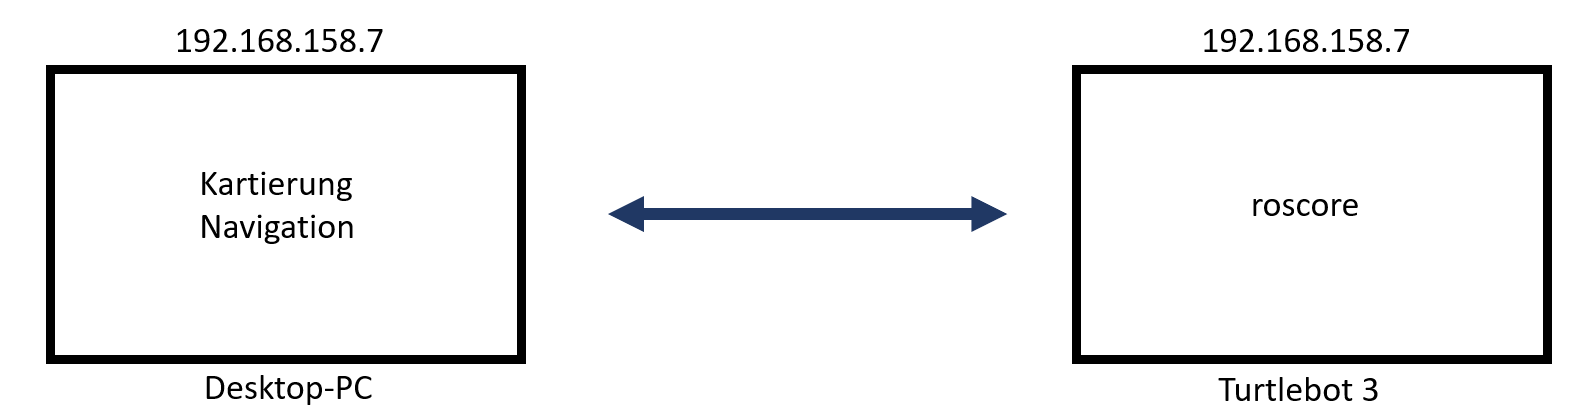
\includegraphics[height=5cm]{Bilder/network_turtlebot.png}
			\caption{Netzwerkverbindung und Programmaufteilung} 
			\label{pic:networkturtlebot}
		\end{figure}
		}
		
		\subsubsection{Simulation und Visualisierung}
		{
			Gazebo ist ein Open-Source-Programm \footnote{Frei zur Verfügung gestellt}, welches eine vollständige Simulation von Robotern, Umgebungen und Messungen ermöglicht. Robotermodelle können dazu modelliert werden, ebenso wie Umgebungen. Der Roboter kann sich daraufhin, wie in der realen Welt, bewegen und Messungen durchführen. Durch eine realistische Physik-Engine\footnote{Virtuelle Simulation physikalischer Kräfte} können Messungen wie in der echten Welt simuliert werden. D.\,h.\ der simulierte Roboter, in meinem Fall der Turtlebot, erhält Messdaten durch seinen Sensor, welche basierend auf der virtuellen Welt errechnet werden. Da ich einen größeren Teil meiner Arbeit von zuhause verrichtet habe, wurde dieses Programm oft genutzt, weshalb auch immer Bilder aus diesem Programm, anstelle von Bildern aus der echten Welt, gezeigt werden.
			
			Rviz ist ebenso ein Open-Source-Tool, welches es ermöglicht, Daten, ob gemessen oder errechnet, zu visualisieren. Dafür empfängt ROS Daten der Nodes und präsentiert diese auf geeigneter Weise. So kann beispielsweise die Momentane Bewegungsrichtung als Pfeil, Messdaten des LiDAR-Sensors als Punkte oder eine Errechnete Karte als Hintergrundbild angezeigt werden
			
			
		}
	}
	\subsection{Turtlebot}
	{
		\subsubsection{Überblick}
		{
			Der Turtlebot ist ein beliebtes Robotermodell der Firma Robotis und kommt in verschiedenen Varianten. Das gute Preis-Leistungs-Verhältnis, sowie die Einsteigerfreundlichkeit, kombiniert mit vielen Integration in andere Programme machen in zu einer guten Wahl für viele Projekte
			Der Turtlebot 3 besteht aus vier Basisplatten, auf welchen die gesamte Technik des Roboters untergebracht ist. Auf der untersten Basisplatte findet man zwei Servomotoren der X-Series von Dynamixel vor, welche dem Turtlebot seine Mobilität verleihen, auf den anderen Plattformen ist ein Raspberry PI 3, welcher unter Umständen auch durch einen Raspberry Pi 4 ersetzt werden kann, sowie ein Einplatinencomputer vorzufinden. Bei Letzterem handelt es sich standardmäßig um einen Intel Joule 570x. Auf der obersten Basisplatte findet man Platz für einen Sensor vor, dort kann eine Kamera, allerdings auch ein Lasersensor oder ähnliches angebracht werden. Auf unserem Turtlebot ist ein LiDAR-Sensor montiert. Dieser Sensor sendet Laserimpulse aus und kann durch das zurückgestrahlte Licht den Raum exakt vermessen. Der Roboter tastet die Umgebung mit den Laserimpulsen ab, was dazu führt, dass er Messpunkte erhält. 
			
			\begin{figure}[H]
				\centering
				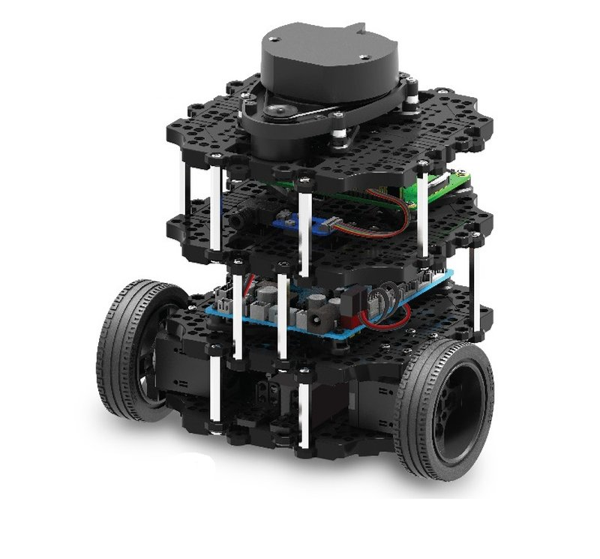
\includegraphics[height=5cm]{Bilder/turtlebot_3_burger.png}
				\caption{Der Turtlebot 3 in der „Burger“ Variante \\ \parencite{turtlebot3burger001}} 
				\label{pic:turtle3burger}
			\end{figure}
			
			%Diese Messpunkte kann der Roboter als Wände oder andere Formen interpretieren. Allerdings handelt es sich dabei um eine 2D Messung, welche in unserem Fall die Umgebung des Roboters auf Höhe des Sensors scannt. Der Sensor kann sich unabhängig vom Roboter um 360° drehen. Ein Problem des Roboters ist, dass er mit dem Standard Sensor keine Hindernisse erkennt, welche nicht auf der Höhe des Sensors sind. Rundum vereint der Roboter eine exzellente Leistung bei günstigen Preisen.
		}
		
		\subsubsection{LiDAR-Sensor}
		{
			Ein LiDAR (Light detection and ranging) - Sensor sendet Laserimpulse aus und kann durch das zurückgestrahlte Licht den Raum exakt vermessen. Der Roboter tastet die Umgebung mit den Laserimpulsen ab, was dazu führt, dass er Messpunkte erhält. Diese Messpunkte kann der Roboter als Wände oder andere Formen interpretieren. Allerdings handelt es sich dabei um eine 2D Messung, welche in unserem Fall die Umgebung des Roboters auf Höhe des Sensors scannt. Der Sensor kann sich unabhängig vom Roboter um 360° drehen. 
			Die Distanz eines Punktes ergibt sich aus der Zeitdifferenz zwischen Aussendung und Empfangen einer elektromagnetischen Welle (Licht) im infraroten Bereich.
			Eine einfache Formel lautet wie folgt:
			
			\begin{equation}
				s = c \cdot \frac{t}{2}
			\end{equation} 
			Hierbei ist $s$ die Entfernung, $t$ die Zeit zwischen Aussendung und Empfangen, sowie $c$ die Lichtgeschwindigkeit.
			
			Ein Problem für Roboters ist, dass mit Hilfe des Standard Sensor keine Hindernisse erkannt werden, welche nicht auf der Höhe des Sensors sind. Dies ist vor allem für Größere Roboter ein Problem, kann aber aufgrund der Umgebung des Roboters, sowie dessen Größen in der Labyrinth-Umgebung vernachlässigt werden.
			\begin{figure}[H]
				\centering
				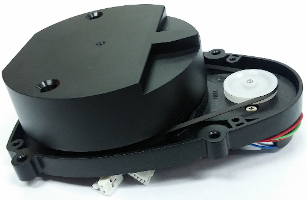
\includegraphics[height=5cm]{Bilder/lds_small.png}
				\caption{Der im Turtlebot 3 verbaute LiDAR-Sensor}
				\label{pic:lds_small}
			\end{figure}
		}
		
		\subsubsection{Raspberrry Pi}
		{
			Auf dem Turtlebot ist ein kleiner Computer, ein der Marke "Raspberry Pi" eingebaut. Standardmäßig handelt es sich dabei um das Modell der Reihe 3, welches jedoch aus Leistungsgründen mit einem Modell der 4. Generation ausgetauscht worden ist. Dieser Mikrocomputer stellt das Herzstück des Roboters dar und steuert alle Vorgänge. Wie ein jeder Computer besteht auch der Raspberry Pi aus einem Prozessor, Arbeitsspeicher, einer SD-Karte als Festplattenersatz und vielem mehr. Zwar stellt die Firma Raspberry auch eine graphische Benutzeroberfläche bereit, jedoch ist diese zur Programmierung nicht notwendig und wird deshalb nicht verwendet, da diese Leistung verbraucht, welche für Berechnungen verwendet werden könnte. Aus diesem Grund verwende ich den Raspberry Pi mit einem einfachen Betriebssystem, welches nur eine Konsole anzeigt, um Leistung zu sparen.
		}
	}
	\subsection{Kartierung}
	{
		\subsubsection{SLAM}
		{
			SLAM (\textit{Simultaneous Localization and Mapping, dt.: Simultane Positionsbestimmung und Kartierung}) beschreibt den Prozess, in welchem eine Karte durch Messdaten erstellt wird, wobei der Roboter selbst auf der Karte verordnet wird.
			Im Fall des Turtlebot geschieht dies mithilfe der Messdaten des LiDAR-Sensors, welcher die Entfernung von Objekten durch Laserstrahlen misst (\textit{siehe LiDAR-Sensor})	
		}
		
		\subsubsection{Positionierung}
		{
			Der Roboter wird anfangs auf den Mittelpunkt der, zu Beginn noch nicht vorhandenen Karte, welche erst durch Messdaten entsteht, platziert. Die Position des Roboters wird entsprechend der Bewegung seiner Motoren kalkuliert. Mithilfe des Umfangs der Reifen kann die bewegte Distanz errechnet werden, da dem Roboter die Winkeländerung der Motoren, z.B. eine Drehung dieser um 180°, bekannt ist. Diese werden an die Motoren übermittelt, wobei die Information noch an andere Teile weitergeleitet werden kann, hier der Microchip auf der Hauptplatine des Raspberry Pi 3 in der Mitte der Roboters, welcher damit Rechnungen, eben zur Positionskorrektur durchführen kann. Vereinfacht gilt daher bei einer geraden Bewegung
			\begin{equation}
				D = R \cdot U
			\end{equation} 
			
			Hierbei steht $D$ für die zurückgelegte Distanz, $R$ für die Umdrehungen der Motoren und $U$ für den Umfang der Reifen. Die Rotation, also die Drehung des Roboters, wird aus der Rotationsdifferenz beider Motoren berechnet. Dreht sich der rechte Motor weiter (größerer Winkel), so dreht sich der Roboter nach links, für eine Rechtsdrehung gilt das Gegenteil.
			Auf diese Weise kann nur aus den Daten, welche an der Motoren gesendet wird, errechnet werden wie weit und in welche Richtung der Roboter sich bewegt hat.
			Die benötigten Daten werden aus Odometrie-Daten gelesen. Dies sind interne Daten des Roboters, welche durch Messungen oder (wie oben genannt) Rechnungen erhält. Diese weichen durch Umwelteinflüsse und Messungenauigkeiten leicht von der Realität ab.
			
			
		\subsubsection{GMapping}
		{
			GMapping beschreibt einen SLAM-Algorithmus, welche an der Universität Freiburg über Jahre hinweg entwickelt worden ist. Dieser ist einer der  meist genutzten Algorithmen für diese Zwecke und deshalb gibt es auch eine Implementation für das Robot-Operating-System. Die Entwicklung eines eigenen Kartierungsalgorithmus geht weit über die Zeitspanne dieses Projektes hinüber, weshalb das GMapping-ROS-Packet verwendet wird (siehe \textit{Kartierung}) %https://people.eecs.berkeley.edu/~pabbeel/cs287-fa11/slides/gmapping.pdf
			
		}
	}

	\subsection{Monte-Carlo-Lokalisation}
	{ 
		Hat ein Roboter eine Karte seiner Umgebung. bringt diese ohne die Position des Roboters in der Karte nicht viel. Die Monte-Carlo-Lokalisation ist eine Möglichkeit, um die Position des Roboters innerhalb der Karte zu bestimmen.  Dafür wird die Karte der Umgebung, sowie die Sensordaten, benötigt. Anfangs ist es gleich wahrscheinlich, dass der Roboter sich in jeglicher Stelle auf der Karte befindet. Nun werden die gemessenen Sensorpunkte und die Karte der Umgebung übereinander gelegt. Stimmen Hindernisse, welche durch die Karte in der Nähe sind, sowie gemessene Sensordaten der realen Welt überein, so ist es wahrscheinlich, dass sich der Roboter an dieser Stelle in der Karte befindet. Misst der Turtlebot beispielsweise einen Runden Gegenstand vor sich und in einer Position auf der Karte ist in gleicher Distanz eine Runde Säule vor dem Roboter, so ist es wahrscheinlich, dass der Roboter sich in dieser Position befindet. Nachdem dieser sich bewegt hat, wird der Vorgang wiederholt, wodurch die möglichen Positionen immer nähe beieinander liegen, da entfernte Schätzungen aufgrund der vielseitigen Umgebung nicht mehr mit den Sensordaten übereinstimmen. 
	}
	\subsection{Wegfindung}
	{
		\subsubsection{Definition}
		{
			Pathfinding (\textit{dt. Wegfindung}) beschreibt den Prozess der Wegfindung, wobei der kürzestmöglichen Weg von einem Startpunkt zu einem Zielpunkt gefunden werden soll. Dieser Prozess setzt eine Karte der Umgebung (\textit{siehe SLAM}), in welcher ein Weg gefunden werden soll, voraus.
		}
		
		\subsubsection{Anwendung in der heutigen Welt}
		{
			Pathfinding-Prozesse sind von heutiger Technologie nicht mehr zu trennen. Sie sind überall präsent und helfen uns, auch wenn wir es manchmal nicht bemerken . Navigationssysteme müssen die kürzeste Route zu einem Zielpunkt finden, wohingegen Staubsaugroboter Orte in einem Haus erreichen müssen. Signale über Satelliten hinweg werden auch über den kürzesten Weg geleitet. Diesen zu finden bedeutet immer, dass für den Transport weniger Aufwand und Zeit benötigt wird
		}
		
		\subsubsection{Algorithmen zur Umsetzung}
		{
			Für die Wegfindung gibt es viele etablierte Algorithmen, jedoch stellt sich nun die Frage, welcher am Nützlichsten ist. Diese Nützlichkeit wird meist an zwei Faktoren gemessen. Diese sind zum einem die Genauigkeit, welche beschreibt ob ein Algorithmus den besten Weg findet, und zum anderen die Geschwindigkeit. Diese beschreibt, wie effizient ein Algorithmus den idealen Weg findet. Mit Geschwindigkeit ist also nicht die Zeit der Ausführung gemeint, welche mit der Effizienz jedoch stark zusammenhängt, da diese je nach genutzten Bauteilen in Computern variiert. Vielmehr wird, wie erwähnt, die Rechenintensität als Maß genutzt. Diese beschreibt, wie viele Schritte durchgeführt werden müssen, bis der ideale Weg gefunden wurde. Je geringer, desto besser. 
			
			Viele Wegfindungsalgorithmen nutzen das gleiche Grundprinzip. Die Karte wird in kleine Vierecke unterteilt. Vom Startpunkt aus wird nun in eine Richtung gegangen und zwar einen Schritt weit. Dabei wird diese Stelle als "besucht" angesehen, wobei von ihr aus nun in weitere Richtungen gelaufen werden kann (Abbildung \ref{pic:pathfinding_procedure_1}). Grenzt eine besuchte Fläche an das Ziel an, so wurde ein Weg gefunden. Nachdem anfangs in jede Richtung ein Schritt in die Tiefe gegangen wurde, wird nun erneut in eine andere Richtung gegangen, bis in jede Richtung ein Schritt gegangen bzw. abgesucht worden ist (Abbildung \ref{pic:pathfinding_procedure_4}). Eine Tiefe (Längeneinheit) wurde somit vollständig abgedeckt. Daraufhin wird nun das Gleiche mit einer Tiefe von zwei zum Startpunkt hin wiederholt wird.
			
			\begin{figure}[H]
				\begin{minipage}{0.5\textwidth}
					\centering
					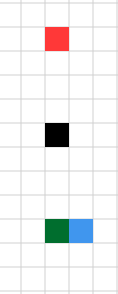
\includegraphics[height=5cm]{Bilder/pathfinding_procedure_1.png}
					\caption{\\ 1. Feld wird durchlaufen} 
					\label{pic:pathfinding_procedure_1}
				\end{minipage}
				\begin{minipage}{0.5\textwidth}
					\centering
					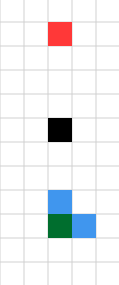
\includegraphics[height=5cm]{Bilder/pathfinding_procedure_2.png}
					\caption{\\ 2. Feld wird durchlaufen} 
					\label{pic:pathfinding_procedure_2}
				\end{minipage}
				\newline
				\begin{minipage}{0.5\textwidth}
					\centering
					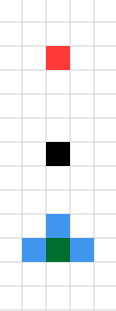
\includegraphics[height=5cm]{Bilder/pathfinding_procedure_3.png}
					\caption{\\ 3. Feld wird durchlaufen} 
					\label{pic:pathfinding_procedure_3}
				\end{minipage}
				\begin{minipage}{0.5\textwidth}
					\centering
					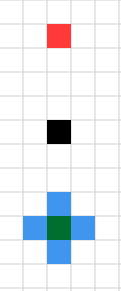
\includegraphics[height=5cm]{Bilder/pathfinding_procedure_4.png}
					\caption{\\ 4. Feld wird durchlaufen}
					\label{pic:pathfinding_procedure_4}
				\end{minipage}
			\end{figure}
			
			
			%evtl \newpage
			Dies wird in der unteren Abbildung verdeutlicht. Grün repräsentiert den Startpunkt, Rot den Endpunkt. Schwarz repräsentiert ein nicht passierbares Feld und blaue Felder sind von dem Suchalgorithmus bereits besucht worden. 
			Die dargestellte Suchart stellt den \textbf{Breadth-first Search Algorithmus} dar, welche zur oben gegebenen Beschreibung passt. Dabei handelt es sich um einen einfachen Wegfindungsalgorithmus.
			
			\begin{figure}[H]
				\begin{minipage}{0.5\textwidth}
					\centering
					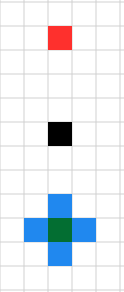
\includegraphics[height=5cm]{Bilder/pathfinding_tiefe1.png}
					\caption{Besuchte Felder nachdem die \\ Tiefe 1 durchlaufen wurde} %\parencite{flora85}}
					\label{pic:pathtiefe1}
				\end{minipage}
				\begin{minipage}{0.5\textwidth}
					\centering
					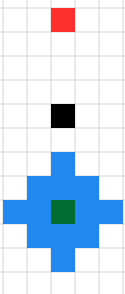
\includegraphics[height=5cm]{Bilder/pathfinding_tiefe2.png}
					\caption{Besuchte Felder nachdem die \\ Tiefe 2 durchlaufen wurde} %\parencite{northFlora190105}}
					\label{pic:pathtiefe2}
				\end{minipage}
			\end{figure}	
			
			Zur Verbesserung der Effizienz nutzen manche Algorithmen weitere Algorithmen, die Schätzalgorithmen, welche man auch Heuristik nennt, die Einfluss darauf nehmen, welche Felder als nächstes besucht werden. Felder, welche in Richtung des Ziels zeigen bzw. sehr wahrscheinlich dorthin führen, werden bevorzugt durchlaufen, Felder, welche vom Ziel weg zeigen, werden hingegen seltener Besucht. Dazu misst der Algorithmus nicht nur die Distanz(Kosten) bis zu einem Punkt, um zu berechnen, ob es sich lohnt, von diesem aus weiter zu suchen, sondern auch die Distanz zum Ziel. Mathematisch kann man dies als zusammengesetzte Funktion verstehen.
			\begin{equation}
				f(x) = g(x) + h(x)
			\end{equation}
			
			Hierbei stellt $g(x)$ die Funktion dar, welche die Kosten(Distanz) vom Startpunkt bis zu einem Punkt $x$ berechnet. $h(x)$ beschreibt die vermutete Distanz von $x$ bis zum Zielpunkt. Beide Ergebnisse zusammen ergeben einen Wert, welcher die Kosten über einen Punkt $x$ zum Zielpunkt errechnet. Dies wird für viele Punkte $x$ berechnet, wobei der nächste Schritt von dem Punkt ausgeht, welcher den niedrigsten Wert (also die geringste, errechnete Distanz) hat.
			Diese Algorithmen sind für viele Verwendungszwecke sehr effizient. Heuristik nutzende Wegfindungsalgorithmen können unter Umständen nachteilig sein, wenn diese in Labyrinthen eingesetzt werden, welche eine hohe Komplexität aufweisen, da Sackgassen, welche nur durch eine Wand vom Ziel getrennt werden, meist durchsucht werden, obwohl sie im Endeffekt nicht Zielführend sind.
			
			\begin{figure}[H]
				\centering
				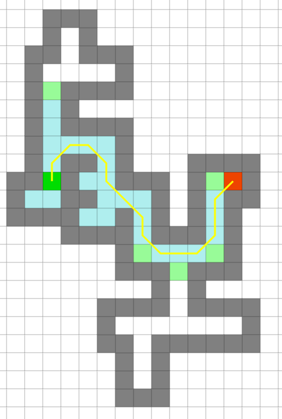
\includegraphics[height=5cm]{Bilder/pathfinding_laby_heu.png}
				\caption{Wegfindung eines Algorithmus mit Heuristik} 
				\label{pic:pathlabheu}
			\end{figure}
		
		
		
		
			\subsubsection{Costmap}
			{
				Die gegebene Karte wird in eine Costmap umgewandelt. Dabei bleibt die Grundfunktion bestehen. Eine Karte, welche Hindernisse aufzeigt. Zusätzlich dazu unterstützt diese Karte jedoch bei der Wegfindung. Jeder Punkt auf der Karte erhält einen Wert - dessen Kost, welche die Wahrscheinlichkeit eines Zusammenstoßes beschreibt. Ist diese Kost hoch, bedeutet dies, dass, sofern der Mittelpunkt des Roboters sich auf diesem Punkt befindet, eine Kollision mit einem Gegenstand sehr wahrscheinlich ist. Je weiter ein Punkt von einem Hindernis entfernt ist, desto geringer ist der Wert dieses Punktes. 
				\begin{figure}[H]
					\centering				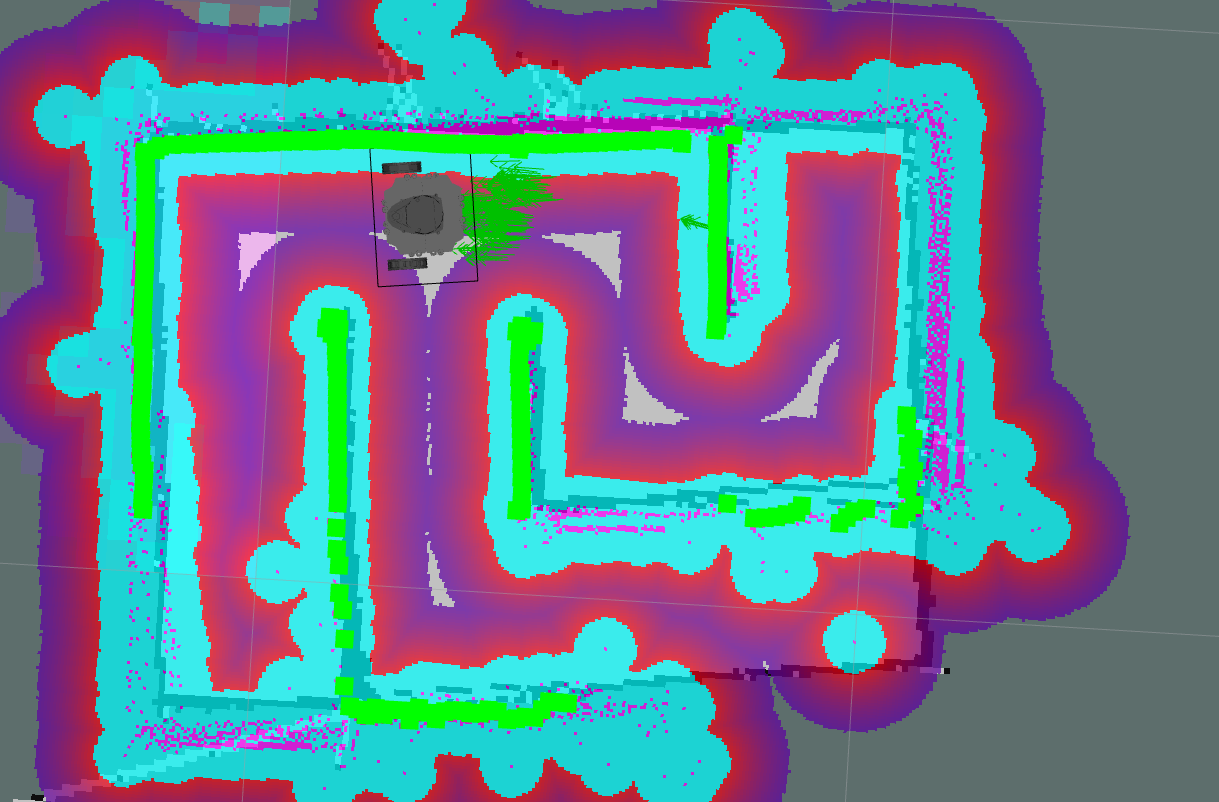
\includegraphics[height=5cm]{Bilder/costmap_overlayed.png}
					\caption{Die Costmap einer Karte} 
					\label{pic:costmapoverlayed}
				\end{figure}
				Die beigefügte Abbildung zeigt die Costmap. Es ist zu erkennen, dass der Bereich um Hindernisse (lila) verschieden gefärbt ist, was die abnehmenden Kosten für diesen Punkt beschreibt.
			}
			
			\subsubsection{Wegplanung}
			{
				Der zu befahrende Weg wird basierend auf mehreren Variablen geplant. Dazu zählt die Distanz im groben, \dahe der kürzeste Weg wird bevorzugt, aber auch gleichzeitig die Wahrscheinlichkeit einer Kollision während des Weges. Dazu werden die Kosten der Punkte auf der Costmap, welche auf dem Weg liegen betrachtet. Um mehr Variabilität bei der Wegplanung zu erlauben, wird die Planung in zwei Bereiche unterteilt. Ein globaler Planer plant den groben Weg zum Ziel, während ein lokaler Planer den Weg entlang des groben Weges plant, wobei gegebenenfalls auch Korrekturen vorgenommen werden müssen.
				
				\begin{figure}[H]
					\centering				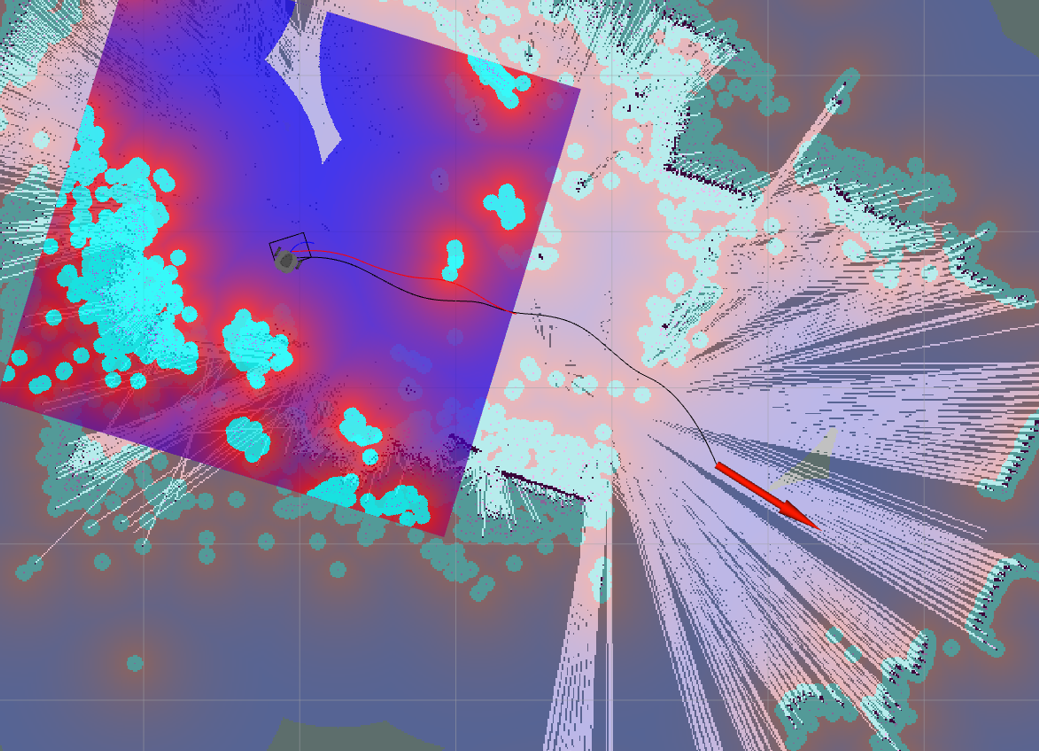
\includegraphics[height=5cm]{Bilder/costmap_pathplanning.png}
					\caption{Die Wegplaning, visualisiert in Rviz} 
					\label{pic:costpathplanning}
				\end{figure}
				
				Die obige Abbildung visualisiert den geplanten Weg. Dieser ist in einen roten, den lokal geplanten Weg, sowie einen Schwarzen, den global geplanten Weg aufgeteilt. Der blaue Strich repräsentiert die momentane Bewegungsrichtung. Weiter ist zu erkennen, dass die Costmap in einen lokalen Bereich (Rechteck), sowie einen globalen Bereich. Der lokale Bereich ist für die kurzfristige Wegplanung (lokaler Planer) für Bedeutung und hebt Hindernisse stärker hervor.
				
			}
			\subsection{Implementierung der Wegfindung} %https://www.researchgate.net/publication/253239158_ROSoClingo_A_ROS_package_for_ASP-based_robot_control
			{
				Um den Roboter nun zu einem Ziel zu navigieren, wird das move\textunderscore base-Packet verwendet. Dieses steuert die Navigation des Roboters, sowie den Pfad, welchem der Roboter folgen soll. Es besteht aus mehreren Nodes (in der Abbildung oval dargestellt).  Dazu abonniert diese Nodes verschiedene Topics. Dazu gehören Sensordaten (z.B. sensor\textunderscore msgs/LaserScan für die Daten des LiDAR-Sensors), Odometriedaten und eine Karte. Die Karte wird durch einen Kartenserver bereitgestellt, welcher, als Node, diese Karte veröffentlicht, sodass jegliche Programme darauf zugreifen können. Dafür muss die Karte jedoch als Bild vorliegen, weshalb die Karte nach vollendeter Kartierung des Labyrinth auf einem Datenträger, meist die Festplatte eines über Wifi mit dem Turtlebot verbundenen Computers, gespeichert werden muss. Die gespeicherte Karte kann daraufhin von dem Karten-Server geöffnet werden. Dieses System sorgt gleichzeitig dafür, dass man eine Umgebung zur Navigation nicht notwendigerweise erneut kartieren muss, sollte schon eine Karte existieren. Im Anwendungsfall ist dies auch praktisch. Staubsaugroboter müssen daher beispielsweise nicht jedes mal erneut eine komplette Karte eines Hauses erstellen.
				\begin{figure}[H]
					\centering
					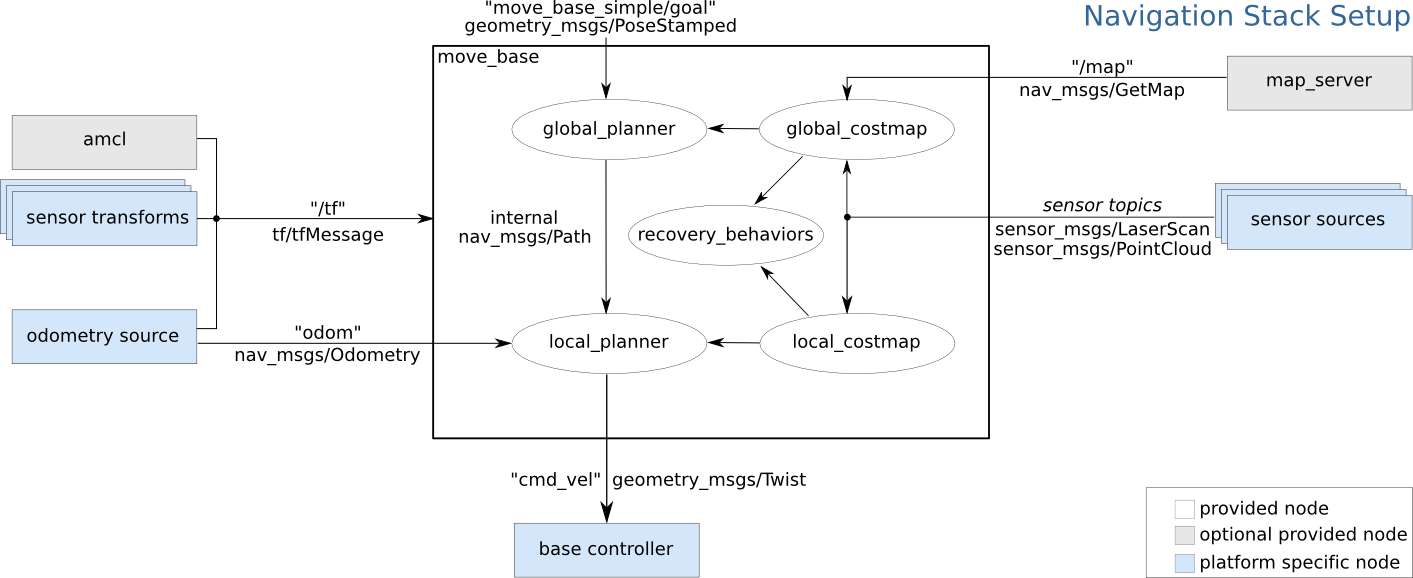
\includegraphics[height=7cm]{Bilder/overview_move_base.png}
					\caption{Das move\textunderscore base-Packet \\
						\parencite{movebasenodeoverview}} 
					\label{pic:overviewmovebase}
				\end{figure}
				
				Nachdem der Roboter nun auf der durch den Kartenserver bereitgestellten Karte verordnet ist, muss dem Roboter ein Navigationsziel gegeben werden.
				Dazu gibt es mehrere Möglichkeiten. Das Programm Rviz ermöglicht es, wie bereits erwähnt, die Karte zu visualisieren. Gleichzeitig hat dies den Nebeneffekt, dass man durch das Programm bestimmen kann, welche Koordinaten ein Punkt auf der Karte hat, indem man die Maus auf diesen Bewegt. Rviz ermöglicht es sogar, direkt im Programm ein Navigationsziel festzulegen, was jedoch teilweise von dem Roboter nicht akzeptiert wird, weshalb ich ein Skript nutze, um die Koordinaten des Zielpunktes, welche ich in Rviz ablesen kann, an das move\textunderscore base-Package zu übertragen.
}

	% !TEXroot=main.tex
\section{Lösungskonzept}
{
	Zur Lösung der Aufgabe wurde ein Turtlebot Roboter benutzt. Dieser ermöglicht durch den Raspberry Pi, welcher eingebaut ist, eine einfache Programmierung. Auf dem Raspberry Pi läuft das Robot-Operating-Systme, was eine einfache Steuerung und Programmierung ermöglicht.
	\begin{figure}[H]
		\centering
		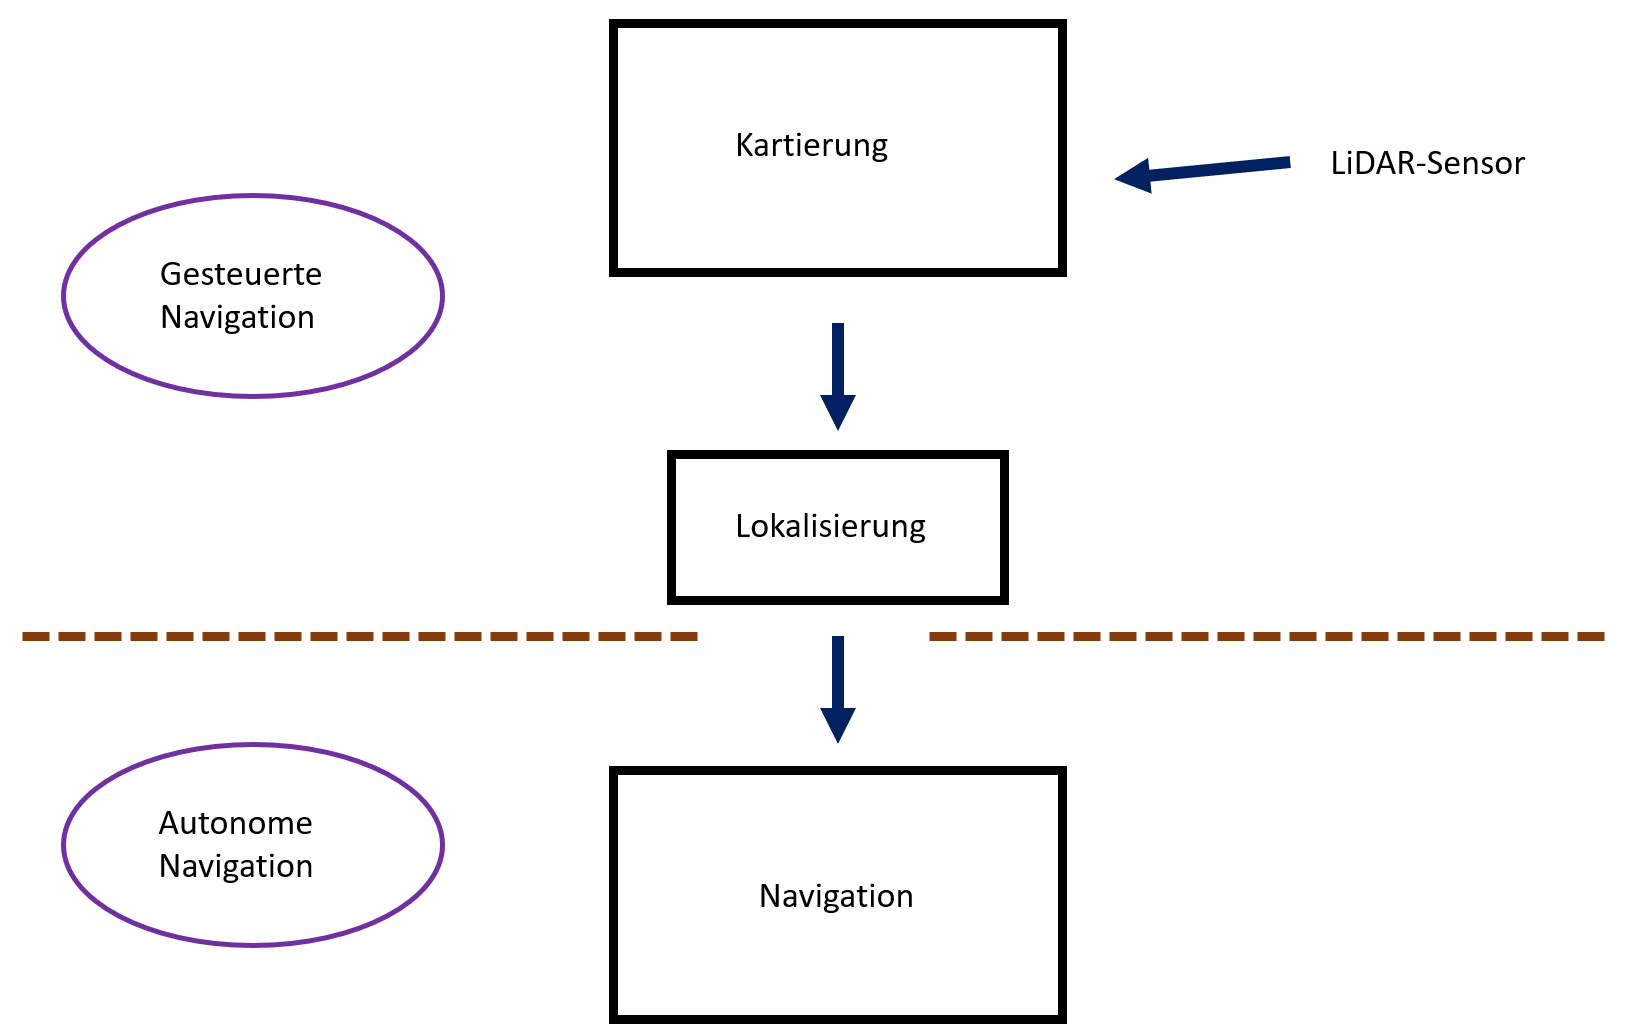
\includegraphics[height=8cm]{Bilder/overview_concept.png}
		\caption{Vorgehensweise zur autonomen Navigation} 
		\label{pic:overviewconcept}
	\end{figure}
Der Roboter wird anfangs mit Hilfe einer Tastatur oder eines Controllers gesteuert. Dabei wird, mit Hilfe des GMapping-Algorithmus, durch die Messdaten des LiDAR-Sensors, eine Karte der Umgebung erstellt. Damit der Karte nicht jedes mal erneut erstellen muss besteht auch die Möglichkeit, eine bereits existierende Karte einzulesen. Auf der erstellten Karte wird der Roboter lokalisiert und positioniert. Sind diese Bedingungen erfüllt, kann der Roboter durch ein Navigationspaket im Labyrinth navigieren, wobei keine Steuerung durch einen Menschen mehr benötigt wird.
}
	% !TEXroot=main.tex
\section{Bedienung}
{
	Damit der Turtlebot ein Labyrinth kartieren kann, muss dieser sich in diesem Bewegen, um es vollends auszukundschaften. Dazu wird sowohl die Tastatur, als auch alternativ ein Logitech Controller verwendet.
	
	\subsection{Steuerung}
	{
		Sowohl die Tastatur, als auch der Controller werden an einen PC angeschlossen. Auf die Eingabe der Tastatur kann sofort zugegriffen werden, jedoch ist im Falle des Controllers mehr Aufwand nötig. Im Falle des Ubuntu-Betriebssystems werden die Eingaben eines Controllers in eine Datei geschrieben, auf welche zugegriffen werden kann. Dabei handelt es sich im Falle des Logitech Controllers um die Datei ``\emph{/dev/input/js0}``.
	}

	\subsection{Implementierung}
	{ Um die Daten der Eingabegeräte zu verarbeiten und schlussendlich als Bewegungsrichtung auszugeben, wird die \emph{teleop-Node} verwendet.Im Falle der Tastatur als Eingabegerät kann mit den Befehl 
		\begin{lstlisting}
roslaunch turtlebot3_teleop turtlebot3_teleop_key.launch
		\end{lstlisting}
	die dazugehörige Node starten. Danach kann der Roboter mit den Tasten W,A,X,D nach vorne, links,  hinten oder rechts beschleunigt werden. Die Taste S setzt die Geschwindigkeit in bestimmte Richtungen zurück.
	\newline
	Im Falle des Controllers ist ein andere Befehl nötig, welcher mehr Informationen übergibt. Hierbei wird sowohl die Datei, welche die Eingaben des Controllers beinhaltet, sowie die Tastenkonfiguration des Controllers übermittelt.
	\begin{lstlisting}
roslaunch teleop_twist_joy teleop.launch 
joy_dev:="/dev/input/js0" joy_config:="xd3"
	\end{lstlisting}
	
	In beiden Fällen werden die Eingaben in Daten der \emph{geometry\textunderscore msgs/Twist} - Form umgewandelt, welche in ROS oft zur Steuerung von Robotern verwendet wird.
	}
}
	% !TEXroot=main.tex
\section{Kartierung}
{
	Bevor der Roboter sich autonom Bewegen kann, muss dieser seine Umgebung erst kennen. Dafür wird von dieser eine Karte erstellt, auf welche später zurückgegriffen werden kann.
	\subsection{Kartierung mit Hilfe des LiDAR-Sensors}
	{
		Die Kartierung erfolgt mithilfe der Daten des LiDAR-Sensors. Dieser misst den Abstand des Roboters in verschiedene Richtungen punktartig. \newline  
		
		\begin{figure}[H]
			\captionsetup{width=.8\linewidth}
			\centering
			\begin{subfigure}[h]{.33\linewidth}
				\centering
				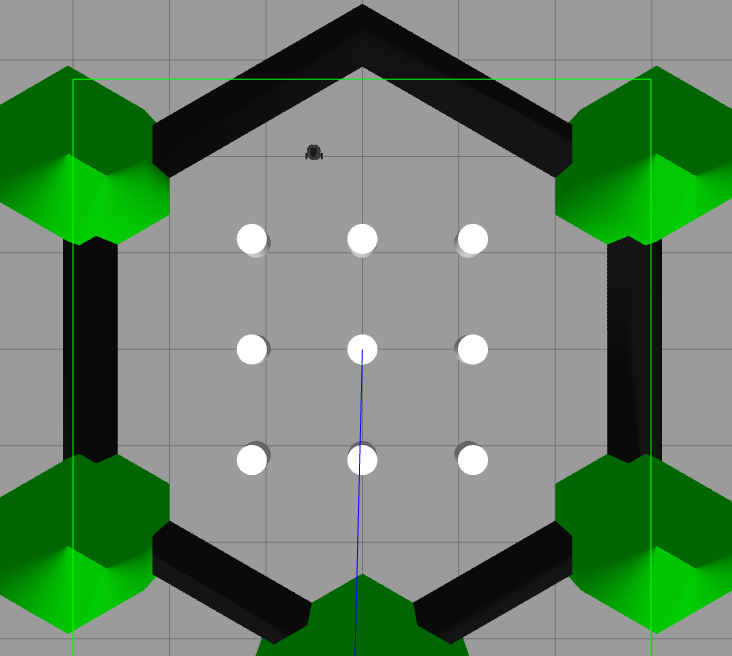
\includegraphics[scale=0.6, height =5cm]{Bilder/virtualmap_world_gazebo.png}
				\subcaption{Roboter (zentriert im oberen Drittel) in einer virtuellen Umgebung}
				\label{pic:virtworldgazebo}
			\end{subfigure}%
			\qquad % erzeugt etwas Abstand
			\begin{subfigure}[h]{.33\linewidth}
				\centering
				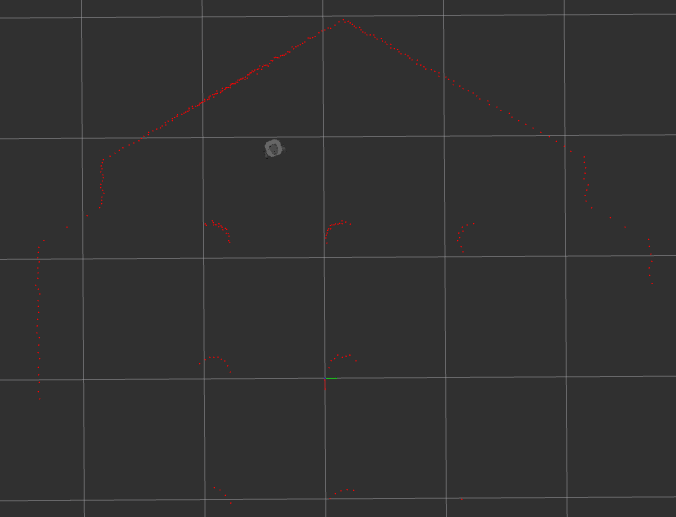
\includegraphics[scale=0.6, height =5cm]{Bilder/virtualmap_world_rviz.png}
				\subcaption{Momentaufnahme der des LiDAR-Sensors gemessenen Punkte (Rot)}
				\label{pic:virtworldlaserrviz}
			\end{subfigure}
			\caption{Eine virtuelle Umgebung und der dazugehörige LiDAR-Scan}
			\label{pic:virtualworld}
		\end{figure}
	
		Links erkennt man eine mit Gazebo simulierte Welt, in welcher sich der Roboter befindet, wobei er von Objekten (Säulen, Mauern) umgeben ist. Das rechte Bild ist ein Ausschnitt aus dem vorher erwähnte Programm Rviz, welches die durch den LiDAR-Sensor gemessene Punkte rot darstellt. Es ist zu erkennen, dass das Verbinden der Roten Punkte auf die Ursprüngliche Umgebung schließen lässt. Je näher der Roboter an einem Objekt ist, desto mehr Punkte befinden sich an dessen Stelle
		
		Zwar gibt eine Messung von einem Standpunkt einen akzeptablen Überblick, so werden jedoch viele Messungen von verschiedenen Stellen benötigt. Durch die Positionsänderung (\emph{siehe Positionierung}) kann errechnet werden wo neue Messpunkte im Vergleich zu alten Messpunkten liegen. Diese Positionierung der Punkte relativ zueinander wird schlussendlich zu einer Karte, wobei viele Messungen nötig sind. Da die Karte jedoch nur aus Punkten besteht, muss der Roboter diese noch interpretieren, sodass viele linear angeordnete Punkte z.B. als Wand interpretiert werden.
		
		Um eine komplette Karte zu erhalten, bewegt sich der Roboter durch die ihm noch unbekannte Welt, bis er eine Region durch genug Messpunkte Kartographiert hat und sich nun in Richtung einer ihm unbekannteren Region bewegen kann. Da der Roboter durch den LiDAR-Sensor konstant seine Umgebung misst, kann die Karte konstant verändert werden, vor allem, wenn der Roboter sich in Richtung weniger erforschte Gebiete bewegt.
		
		Während des Anfangs des Projektes wurde der Roboter noch mit Hilfe der Tastatur an einem Rechner oder über einen Logitech-Controller Gesteuert. Danach wurde daraus jedoch eine autonome Navigation, meist in Richtung von Gebieten, welche weniger erforscht sind. 
		
		Die Kartierung erfolgt mit Hilfe des \emph{GMapping}-Algorithmus. Dieser schaut sich die gescannten Laserdaten der \emph{sensor\textunderscore msgs/LaserScan}-Topic an und veröffentlicht drei Datenarten.
		\begin{enumerate}
			\item ein "Occupancy-Grid": 2D-Karte. Jeder Ort (Pixel) hat einen Ja/Nein Wert, welcher beschreibt, ob sich an der Position ein Objekt befindet oder nicht
			\item Entropie (Sicherheit über die Erkenntnis verschiedener Punkte: unsichere Punkte werden wahrscheinlicher geändert)
			\item Metadaten über die Karte.
		\end{enumerate}
		
		Durch die Kartierung dieses Algorithmus wird aus den einzelnen Laserscan-Daten nun eine Karte. Dies wird in den unteren Abbildungen dargestellt. Hierbei handelt es sich um die Kartierung der in Abbildung \ref{pic:virtworldgazebo} gezeigten Umgebung. Schwarze Punkte wurden als Hindernis erkannt, graue Stellen sind hindernisfreie Punkte. Die durch den LiDAR-Sensor gemessenen Punkte werden in grüner Farbe über die Karte gelegt. In Abbildung \ref{pic:mapping_smpl_2} und \ref{pic:mapping_smpl_3} ist zu erkenne, dass schwarze Punkte nicht direkt mit Gemessenen Punkten des Lasers (grün) übereinstimmen. Dies liegt zum einen darin, dass die Berechnung der Karte Zeit benötigt, weshalb die Punkte noch verarbeitet werden, sowie daran, dass die Aktualisierungsrate der Karte eingestellt werden kann. Während intuitiv eine schnelle Aktualisierungsrate sinnvoll wirkt, ist eine zu hohe Rate nachteilig, da viel Leistung benötigt wird und mehr Fehler gemacht werden, da ungenaue Messpunkte zu schnellen Schlüssen auf der Karte führen. Bei einer längeren Zeitdauer zwischen Kartenaktualisierungen können nämlich mehr gemessene Punkte in Betracht gemessen werden.
		
	
		\begin{figure}[H]
			\captionsetup{width=.8\linewidth}
			\centering
			\begin{subfigure}[h]{.33\linewidth}
				\centering
				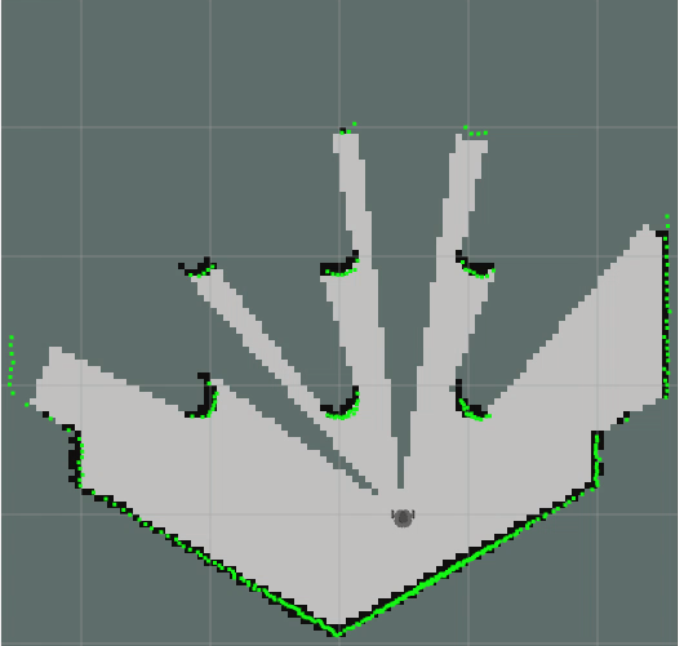
\includegraphics[scale=0.6, height =5cm, width=5cm]{Bilder/mapping_smpl_1.png}
				\subcaption{Kartierung am Anfangspunkt}
				\label{pic:mapping_smpl_1}
			\end{subfigure}%
			\qquad % erzeugt etwas Abstand
			\begin{subfigure}[h]{.33\linewidth}
				\centering
				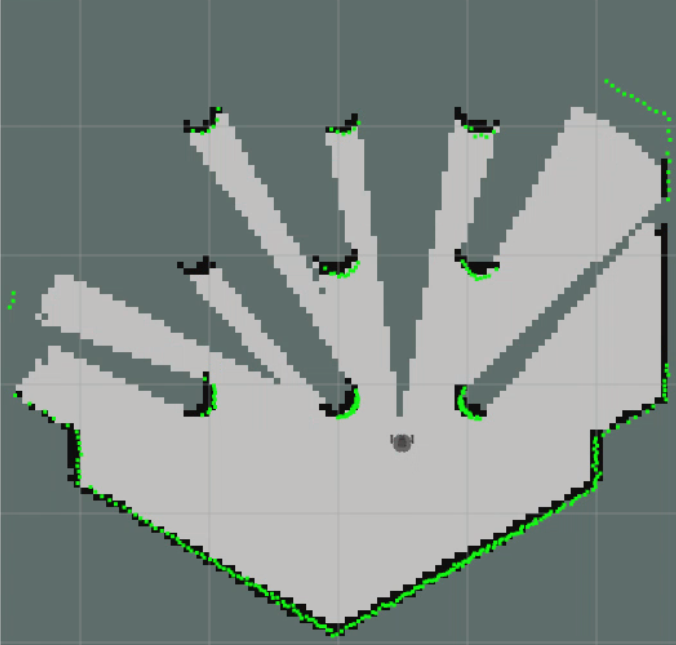
\includegraphics[scale=0.6, height =5cm, width=5cm]{Bilder/mapping_smpl_2.png}
				\subcaption{Kartieruing nach erster Bewegung (nach oben)}
				\label{pic:mapping_smpl_2}
			\end{subfigure}\hfill
			\begin{subfigure}[h]{.33\linewidth}
				\centering
				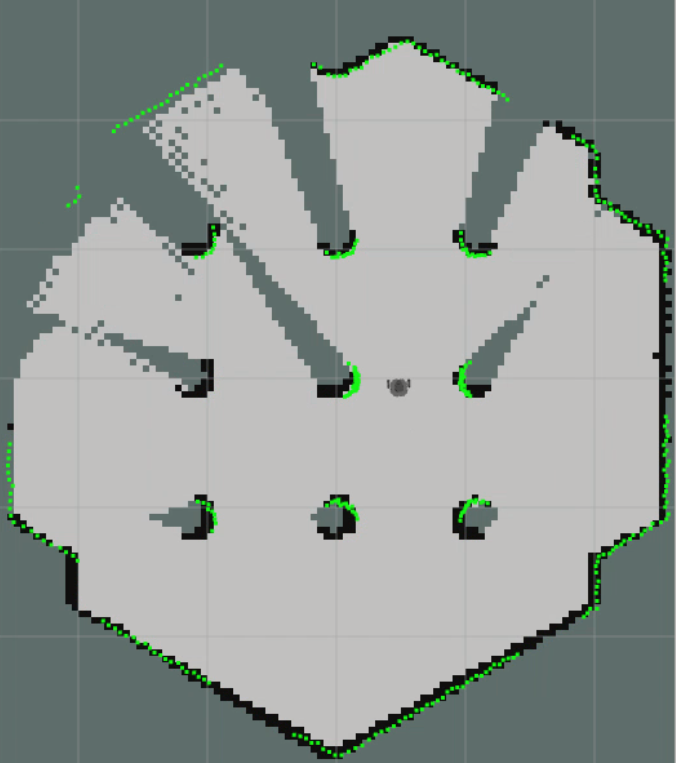
\includegraphics[scale=0.6, height =5cm, width=5cm]{Bilder/mapping_smpl_3.png}
				\subcaption{Kartierung nach weiterer Bewegung}
				\label{pic:mapping_smpl_3}
			\end{subfigure}%
			\qquad % erzeugt etwas Abstand
			\begin{subfigure}[h]{.33\linewidth}
				\centering
				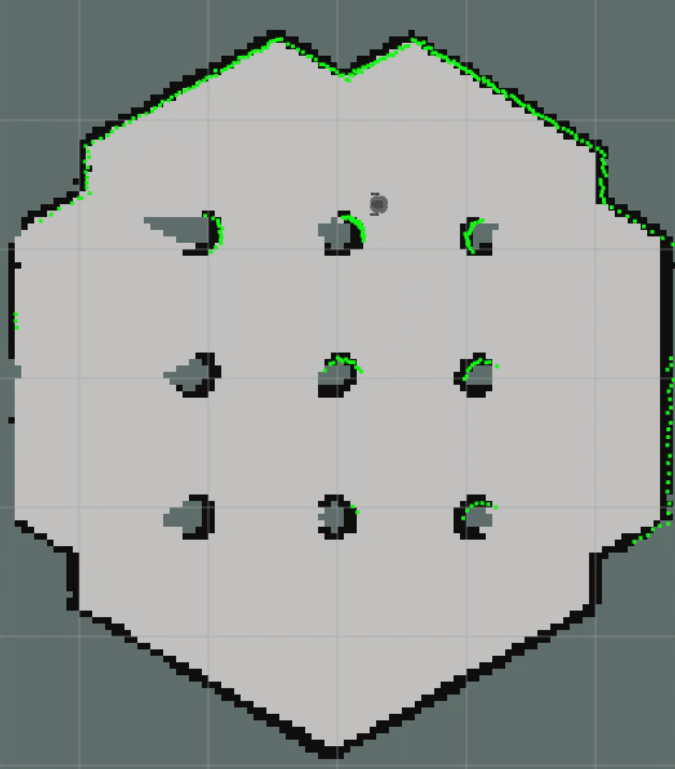
\includegraphics[scale=0.6, height =5cm, width=5cm]{Bilder/mapping_smpl_4.png}
				\subcaption{Kartierung nach Erreichen des oberen Endes}
				\label{pic:mapping_smpl_4}
			\end{subfigure}%
			\caption{Kartierung einer virtuellen Umgebung}
			\label{pic:mapping_smpl}
		\end{figure}
	}
	\subsection{Implementierung}
	{
		Um die Kartierung vor zu nehmen, wird der GMapping, welcher bereits ausgeführt wurde, genutzt. Jedoch müssen einige Parameter angepasst werden, da die Kartierung innerhalb des Labyrinths auf vergleichbar kleinem Raum geschieht. Zuerst wird die Frequenz erhöht, sodass die Karte häufiger, basierend auf den neuen Messdaten, geändert bzw. erneuert wird. Dies wird durch den Parameter $map_update_interval$ bestimmt, welcher auf $6$ gesetzt wird (niedrigerer Wert = niedrigere Periodendauer, woraus eine höhere Frequenz folgt). Gleichzeitig ist zu beachten, dass sich der Roboter auch schnell drehen bzw. bewegen kann. Deshalb müssen Parameter angepasst werden, welche beschreiben, nach welcher zurückgelegten Distanz bzw. Drehung die Karte ebenfalls erneuert wird. Beide Werte werden vergleichsweise niedrig gesetzt, damit die Karte, vor allem bei höheren Geschwindigkeiten oder Drehungen, häufig aktualisiert wird, damit inkorrekte Neupositionierungen oder gar falsche Annahmen über die Umgebung verhindert werden. Dazu wird der $linearUpdate$ Parameter auf $0.05$ und der $angularUpdate$ Parameter auf $0.05$ gesetzt.
		
		Durch den unteren Befehl wird der \emph{GMapping} - Node gestartet.
		\begin{lstlisting}
roslaunch turtlebot3_slam turtlebot3_slam.launch slam_methods:=gmapping
		\end{lstlisting}

	}	

	\subsection{Karten speichern}
	{
		Um einen Raum nicht jedes mal erneut kartieren zu müssen, können Karten auch gespeichert werden. Dafür wird das \emph{map\tus server} - Paket verwendet. Dieses ermöglicht durch den Befehl 
		\begin{lstlisting}
rosrun map_server map_saver -f *path*
		\end{lstlisting}
	das Speichern von erstellten Karten, wobei \emph{*path*} durch Speicherort und Dateinamen ausgetauscht werden muss. Mit Hilfe des Befehls
		\begin{lstlisting}
rosrun map_server map_server  *path.yaml*
		\end{lstlisting}
	kann eine Karte veröffentlicht (gepublished) werden, woraufhin sie für andere Nodes frei verfügbar ist. Auch hier muss \emph{*path*} druch den Pfad der Datei, gefolgt von dem Dateinamen mit der \emph{.yaml} - Endung, ersetzt werden.
	}
}
	% !TEXroot=main.tex
\section{Lokalisierung}
{	
	Sollte man eine eine Karte nutzen, auf welcher der Roboter seine Position noch nicht kennt, so muss der Roboter erst Lokalisiert werden, damit diese auf der Karte verordnet werden kann.
	\subsection{Positionierung auf einer Karte}
	{
		
	Für diesen Prozess wird die Monte-Carlo-Lokalisation verwendet. Als Messpunkte dienen die Daten des LiDAR-Sensors. In Abbildung \ref{pic:costmontecarlo} wird das vergleichen von Sensordaten und Karte deutlich.
		\begin{figure}[H]
			\centering
			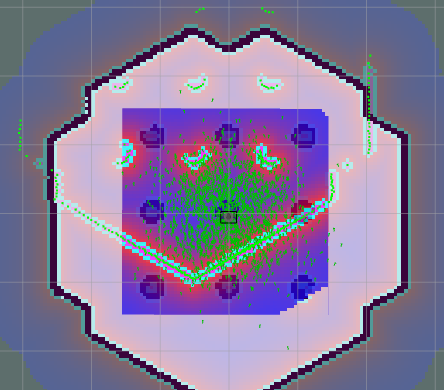
\includegraphics[height=5cm]{Bilder/costmap_monte_carlo_example.png}
			\caption{Costmap mit Sensordaten} 
			\label{pic:costmontecarlo}
		\end{figure}
		In der Abbildung wird deutlich, dass der Roboter auf der gegebenen Karte (Hintergrund) mittig platziert wird. Gleichzeitig misst der LiDAR-Sensor auch Hindernisse, welche wiederum eine neue Karte der Umgebung bilden. Diese Hindernisse sind hell im Vordergrund zu sehen. Man erkennt, dass diese nicht übereinander liegen und der Roboter deshalb noch nicht korrekt positioniert ist. In Wirklichkeit werden Daten aus der unteren linken Ecke der Karte gemessen. Dadurch werden Positionen in dieser Umgebung sehr wahrscheinlich. Damit der Roboter bei vielen ähnlichen Stellen, was hier nicht der Fall ist, trotzdem korrekt positioniert ist, wird der Roboter zwischen verschiedenen LiDAR-Messungen bewegt. Während der Bewegungen wird errechnet, wo der Roboter sich, ausgehend von den ursprünglichen Vermutungen der Position, befindet. Stimmen auch die neuen Messungen mit der Karte überein, so wird eine Position immer wahrscheinlicher, bis der Roboter schlussendlich, sicher positioniert werden kann, da Sensordaten und Karte übereinstimmen. im Falle anderer Roboter können neben LiDAR-Sensoren auch andere Sensordaten verwendet werden.
		
		Die vermuteten Punkte werden dann veröffentlicht, sodass die Navigation darauf zugreifen kann. Diese übermittelten Punkte können in Rviz graphisch dargestellt werden. In Abbildung \ref{pic:amclclearpos} erkennt man im Hintergrund die erstellte Karte, den Laserscan als grüne Punkte und die geschätzten Positionen (Particlecloud) als grüne Pfeile.
		
	\begin{figure}[H]
		\centering
		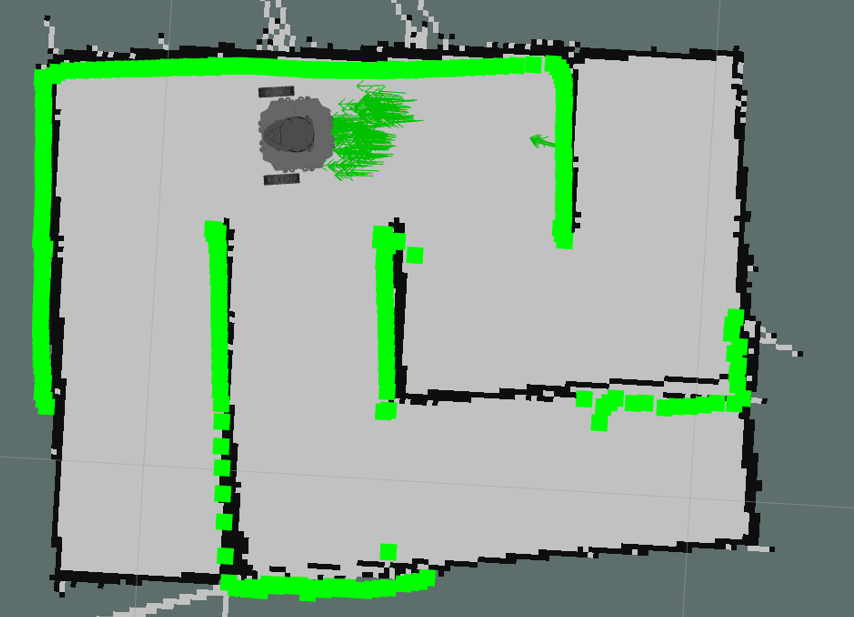
\includegraphics[height=5cm]{Bilder/amcl_clear_pointcloud.png}
		\caption{Particlecloud} 
		\label{pic:amclclearpos}
	\end{figure}

	Es ist zu erkennen, dass gegen Ende der Lokalisierung  die möglichen Positionen eng beieinander sind. Je enger beisammen, desto genauer die Lokalisierung. Die möglichen Positionen werden als Pfeile angezeigt.
	}

	\subsection{Implementierung}
	{
		Die Lokalisierung erfolgt durch das \emph{amcl}-Paket. Dabei handlet es sich um einen Monte-Carlo-Algorithmus. Dieses verwendet die Laserscan-Daten unter der ROS-Topic \emph{/scan}. Dieses Topic beschreibt die Laserscan-Daten welche gemessen werden. Ausgegeben wird das \emph{/particlecloud} Topic, welches die möglichen Positionen beschreibt, welche von der Navigation (siehe Abschnitt 7) genutzt werden.
	}
}
	% !TEXroot=main.tex
\section{Navigation}
{	
		Nachdem der Roboter nun auf der durch den Kartenserver bereitgestellten Karte verordnet wurde, muss dem Roboter ein Navigationsziel gegeben werden, damit eine Route zu diesem Punkt berechnet werden kann. Daraufhin soll der Roboter autonom zu diesem Punkt navigieren. Dieser Abschnitt stellt den letzten Schritt des Projekts dar.
		
		\subsection{Navigationsziel festlegen}
		{
			Rviz bietet dazu eine einfache Möglichkeit. In der oberen Leiste kann die Option ``\emph{2D Nav Goal}`` genutzt werden, um graphisch auf der vorliegenden Karte eine Zielposition festzulegen. Diese wird durch einen Pfeil repräsentiert und beinhaltet auch die Blickrichtung (Abbildung \ref{pic:rviznavgoalsmall}).
			\begin{figure}[b]
				\centering
				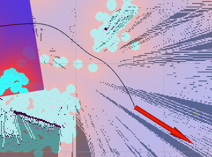
\includegraphics[height=5cm]{Bilder/rviz_navgoal_small.png}
				\caption{Eine in Rviz gesetzte Zielposition} 
				\label{pic:rviznavgoalsmall}
			\end{figure}
		Diese Position wird durch Rviz unter dem \emph{move\textunderscore base\textunderscore simple/goal} - Topic als Nachricht des  \emph{geometry\textunderscore msgs/PoseStamped} - Typs veröffentlicht und damit an die \emph{move\textunderscore base} weitergegeben.
		}
	
		\subsection{Implemention}
		{
			
			
			Die Navigation und Wegplanung geschieht durch das \emph{move\tus base}- Paket. Dabei wird zuerst, wie erwähnt, der grobe Weg, gefolgt von dem exakten Weg im lokalen Bereich berechnet. Dabei wird die durch GMapping erstellte Karte zur Hilfe genommen. Die beigefügte Abbildung  gibt einen Überblick über alle aktiven Nodes. Hierbei stellt das große Rechteck (links) die Komponenten der \emph{move\tus base} dar (Abbildung \ref{pic:rosgfullfront}).
			

			
			Wichtig sind für die Wegplanung hierbei die Parameter der Costmap, da dieser darüber entscheiden, wo der Weg entlang läuft. Dabei spielt das Aufblasen (Inflation) von Hindernissen eine wichtige Rolle. Je stärker ein Objekt aufgeblasen wurde, desto weiter wird es umfahren. Zwar ist ein großer Abstand gut, um Kollisionen zu verhindern, jedoch kann ein Labyrinth nicht viel Platz zwischen den Wänden bieten. Daher können Hindernisse auch nicht so stark aufgeblasen werden. Der Parameter $inflation_radius$ in der Konfigurationsdatei der Costmap beschreibt diesen Wert. Um in dem Labyrinth überhaupt navigieren zu können, ohne dass der Roboter anhält, da er sich im Radius der aufgeblasenen Hindernisse befindet, muss der Wert schon niedrig ($\approx 15\si{cm}$) angesetzt werden. Um das fahren von Kurven zu ermöglichen wurde der Wert auf $10,7 \si{cm}$ gesetzt, was nur $2 \si{mm}$ über dem Roboterradius ist. Dadurch ist der Roboter jedoch in der Lage, in dem Labyrinth weitestgehend problemlos zu navigieren.
			
			Um dem Roboter das befahren von Kurven zu ermöglichen, nutzt man eine funktionalisiert des Turtlebot3-Burger. Dieser kann sich nämlich auf der Stelle drehen. Dadurch muss eine Drehung keinen, vor allem keinen großen Radius haben. Durch das setzten des $min_vel_theta$ Parameters auf $0$, brauch der Roboter für Drehungen nun keine Geschwindigkeit mehr, sondern kann sich im Stand drehen.
			
			\begin{landscape}
				\begin{figure}[htbp]
					\centering
					\fbox{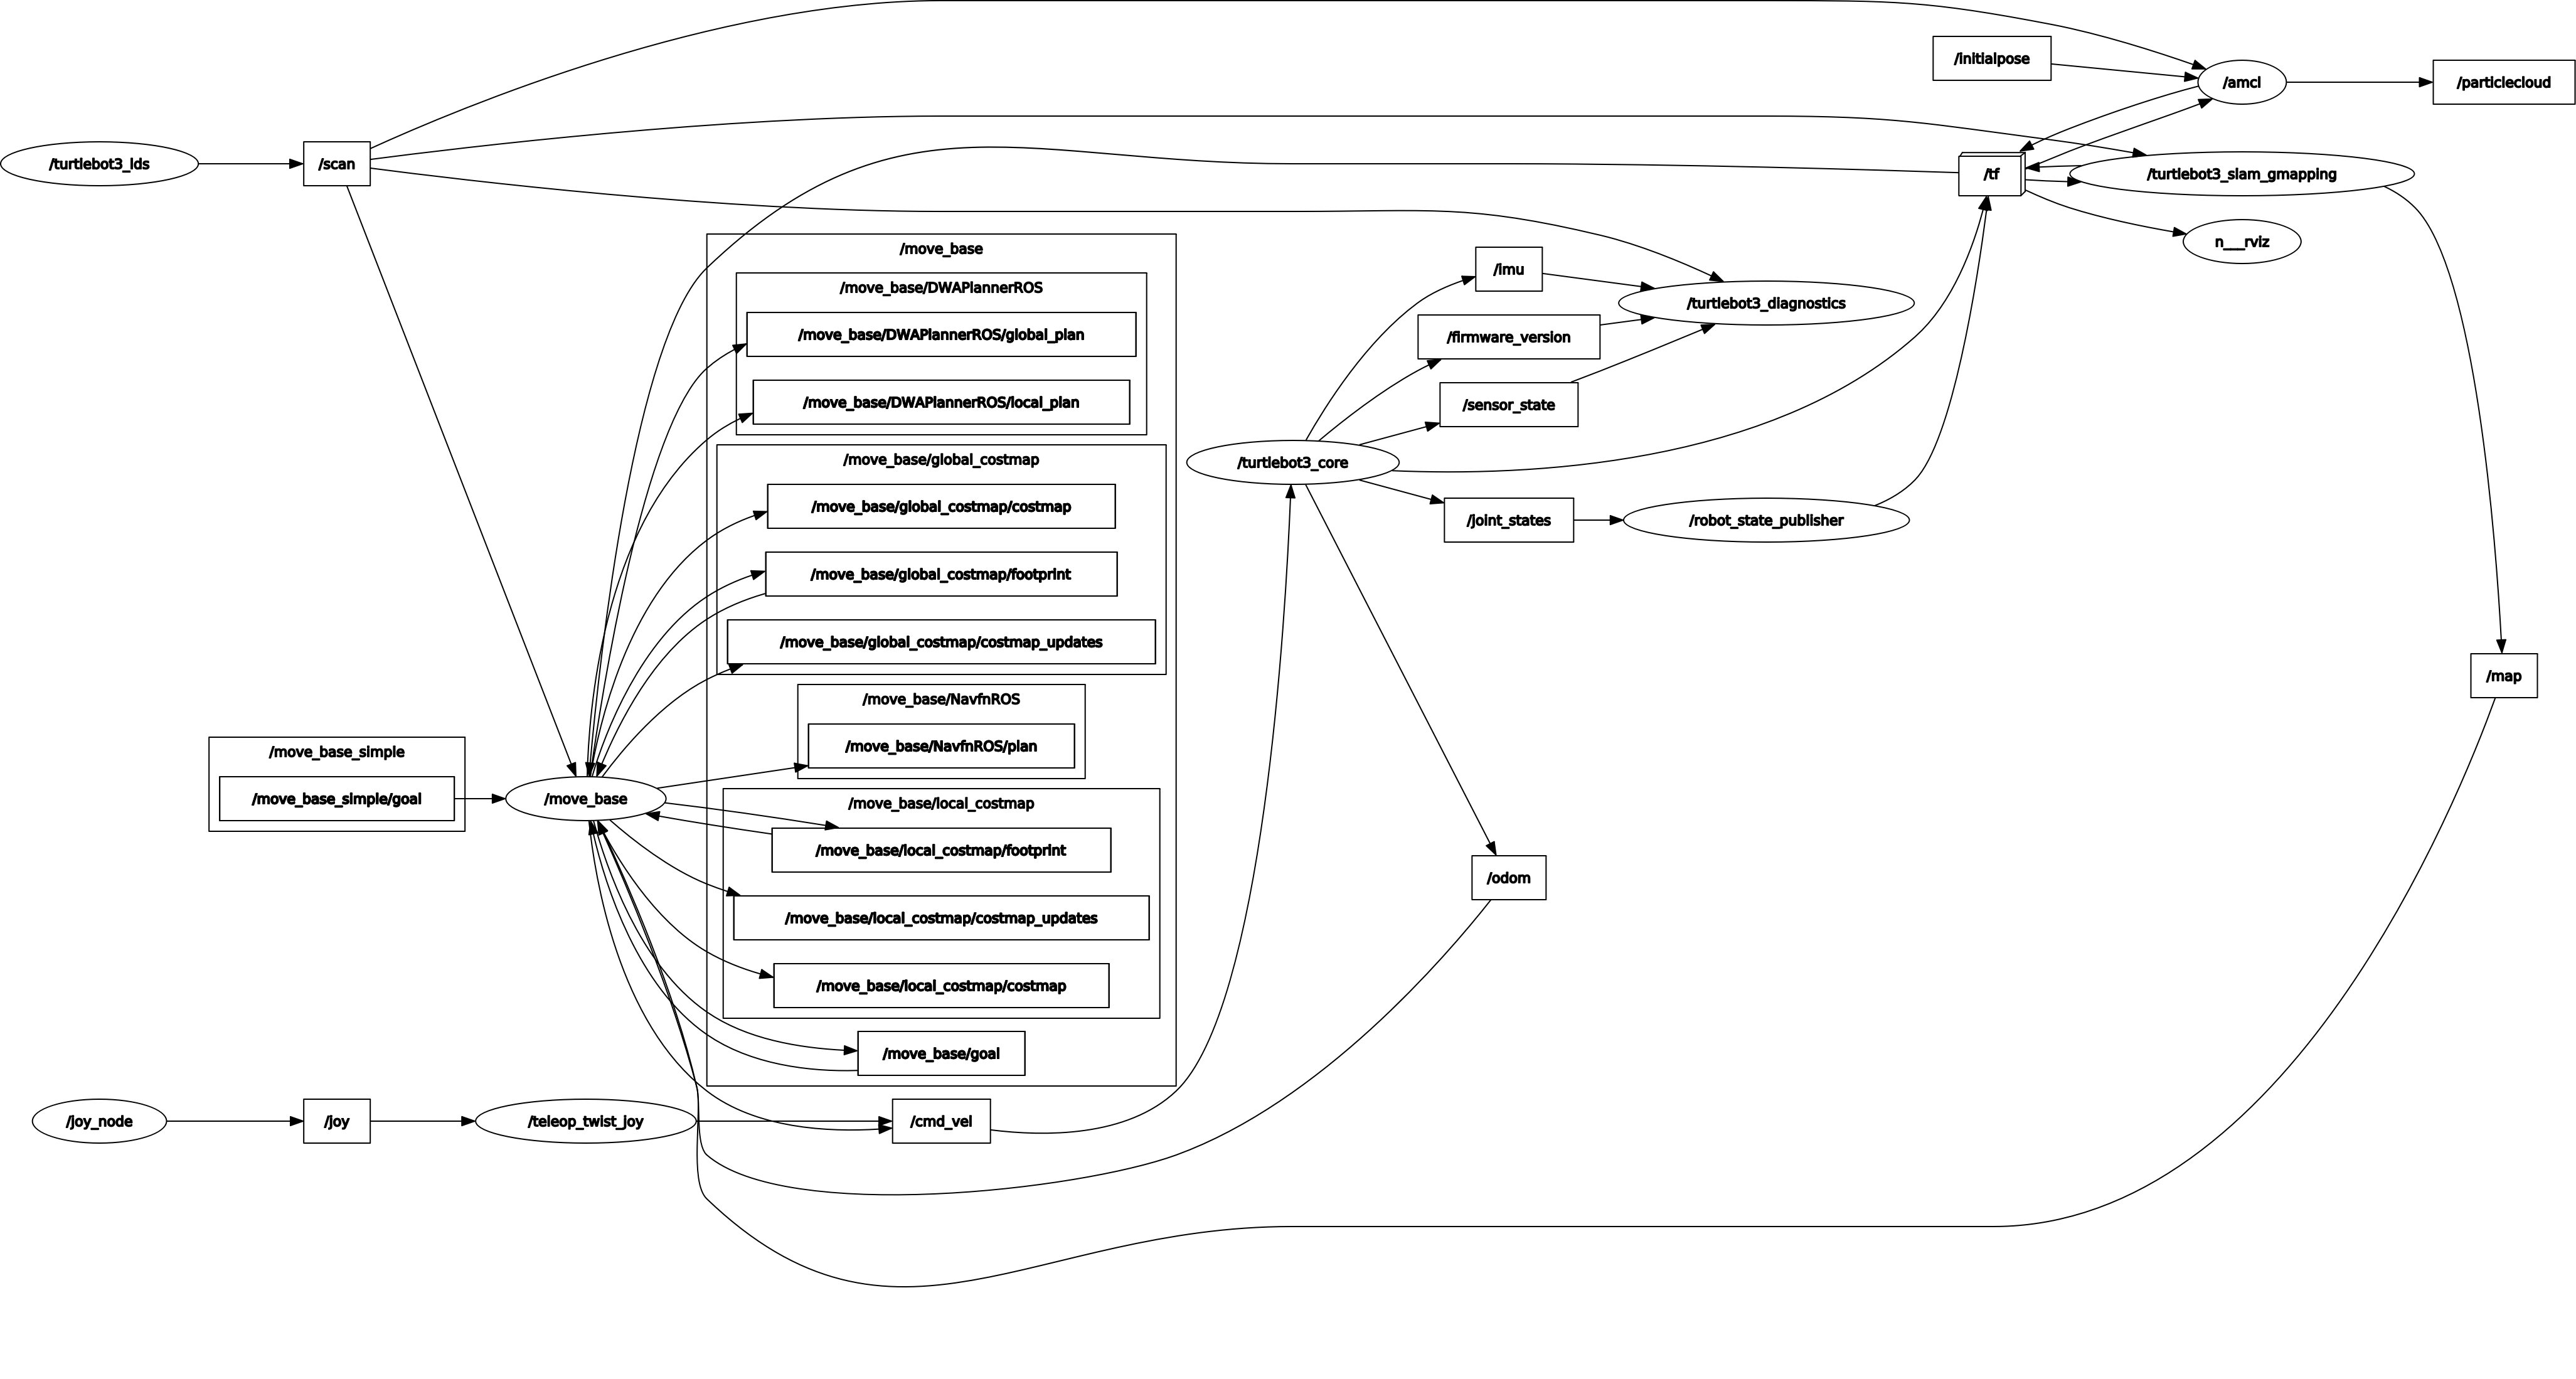
\includegraphics[width=\linewidth, height=\textheight,keepaspectratio]{Bilder/rosgraph_frontier_full.png}} %svg nicht möglich
					\caption[short]{Der gesamte Graph aller aktiven Nodes}
					\label{pic:rosgfullfront}
				\end{figure}
			\end{landscape}

			
			
		}
}	
	% !TEXroot=main.tex

\section{Probleme}
{
	Natürlich gab es während des Projektes auch immer wieder Probleme und Hindernisse, auf welche im Folgenden eingegangen werden.
	\subsection{Bedienung}
	{
		Bei der Bedienung war vor allem die fehlende Dokumentation für den Controller und dessen Einstellung das Problem. Dadurch musste erst herausgefunden werden, auf welcher Gerätedatei (js0) dieser zu finden war. Gleichzeitig war die Konfiguration etwas kontraintuitiv, da die Steuerung durch zwei verschiedene Joysticks geschieht und gleichzeitig ein Knopf gedrückt werden muss.
	}

	\subsection{Kartierung}
	{
		Im Falle der Kartierung war vor allem das finden passender Parameter das Problem. Dabei war die Karte oft ungenau und es gab Verbindungen zwischen Pfaden, welche in Realität keine haben (die Karte verschmilzt). Dies musste durch die schnelle Aktualisierungsrate ausgeglichen werden.
		Ein weiteres kleineres Hindernis war, herauszufinden, dass Studenten den LiDAR-Sensor falsch herum auf den Roboter gebaut haben, wodurch der Roboter sich auf der Karte in eine andere Richtung bewegt hatte, als er in der Realität tat. Dies führte zu seltsamen Karten, konnte aber schlussendlich durch das Umbauen (Drehen) des LiDAR-Sensors gelöst werden.
	}
	
	\subsection{LiDAR-Sensor}
	{
		Der LiDAR-Sensor ist hat teilweise einige Probleme. Durch Reflexion des ausgestrahlten Lichtes im richtigen, meist steilen Winkel entstehen Punkte auf der Karte, welche als Hindernisse erkannt werden, aber keine sind. Diese finden sich auch auf der Costmap wieder. Da die Fehlmessungen konstant reproduzierbar waren und damit nicht zufällig erfolgten, konnte das Problem teilweise gelöst werden. Indem die Auflösung der Costmap verringert wurde. Dadurch beschreibt ein  Pixel einen größeren Bereich in der echten Welt und kleine Fehlmessungen werden ausradiert, da die benachbarten Punkte nicht als Hindernis erkannt werden. Trotzdem kam es immer wieder zu solchen Reflexionsfehlern.
	}

}
\newpage
\section{Zusammenfassung}
{
	Schon im heutigen Zeitalter ist die Navigation von Robotern in einer unbekannten Umgebung eine Sache der Möglichkeit. Mit Hilfe von Algorithmen, wie \zb GMapping, an deren Entwicklung viele Beteiligt waren, ist es möglich, eine Karte zu erstellen, indem man die Vorteile der Veröffentlichung von Open-Source-Paketen nutzt. Noch dazu bietet ROS ein ideales Grundprinzip, in welchem Komponenten schnell integriert und ausgewechselt werden können. So kann die Kompatibilität vieler Komponenten gewährleistet werden. Nicht zuletzt deshalb gibt es Pakete für den Turtlebot, welche diesen vereinfacht ansteuern lassen und eine Integration einer Pfadplanung, so \zb durch die move\textunderscore base, welche in vielen Robotern genutzt werden kann.
	Die nächsten Schritte für dieses Projekt wären möglicherweise eine Kamera, welche, ähnlich zu dem ``RoboCup-Maze`` Bilder bzw. Symbole an den Wänden des Labyrinthes erkennt und nach diesen handelt, was auch Möglichkeiten für kleinere Anbauten an den Roboter, wie \zb eine Taschenlampe oder einen Greifarm, liefert.
	%ROS-Komponenten in Grundlagen - ROS
}
	
	\printbibliography[heading=bibintoc]
\end{document}